\chapter{Μέθοδος}
\label{chap:method}

Όπως αναφέραμε στο προηγούμενο κεφάλαιο, οι θεμελιακές υλοποιήσεις των νευρωνικών δικτύων από κάψουλες (\cite{hinton2011transforming, sabour2017dynamic, hinton2018matrix}) βασίζονται σε υποθέσεις των οποίων η εγκυρότητα δεν έχει δοκιμαστεί εκτενώς. Για τον λόγο αυτό (αλλά και για λόγους σύγκρισης με άλλες μεθόδους), δύο από τις τέσσερεις μεθόδους που χρησιμοποιούμε στο πειραματικό μέρος της παρούσας διπλωματικής αναπτύχθηκαν (ή τροποποιήθηκαν) σε πηγαίο κώδικα σύμφωνα με την αρχιτεκτονική και τον αλγόριθμο δρομολόγησης που παρουσιάζονται στα έργα \cite{sabour2017dynamic} και \cite{hinton2018matrix} αντίστοιχα. \par

Οι δύο τελευταίες μέθοδοί του παρόντος κεφαλαίου, πατώντας στις βασικές δομικές αρχές των νευρωνικών δικτύων με κάψουλες, επιδιώκουν να βελτιώσουν ορισμένες από τις ανεπάρκειες της τεχνολογίας. Έτσι, προτείνονται καινοτόμοι αλγόριθμοι και αρχιτεκτονικές νευρωνικών δικτύων που εστιάζουν είτε σε προβλήματα ταχύτητας και κλιμακωσιμότητας (τρίτη μέθοδος) είτε στα προβλήματα εγκυρότητας των αρχικών υποθέσεων (τέταρτη μέθοδος).


\section{\en{Dynamic Routing Between Capsules}}

Η μέθοδος της \textquote{Δυναμικής Δρομολόγησης με Κάψουλες} υλοποιήθηκε σε κώδικα ακολουθώντας πιστά την ομώνυμη δημοσίευση των \en{Sabour S. et al.} \cite{sabour2017dynamic}. Αν και υπήρχαν έτοιμες υλοποιήσεις του έργου στο διαδίκτυο, δυστυχώς ο κώδικάς τους ήταν αναχρονισμένος και δε λειτουργούσε σε σύγχρονα συστήματα με τις νέες εκδόσεις των πακέτων λογισμικού. Για αυτό και υλοποιήθηκε εκ νέου στη γλώσσα \en{python 3} χρησιμοποιώντας τη βιβλιοθήκη \en{tensorflow 2}. \par

Σε αυτήν την ενότητα θα ξεκινήσουμε παρουσιάζοντας τη γενική αρχιτεκτονική του νευρωνικού δικτύου με κάψουλες που προτείνει το εν λόγω έργο. Στη συνέχεια και σε ξεχωριστή υπο\textendash ενότητα θα παρουσιάσουμε τον αλγόριθμο δρομολόγησης που λαμβάνει χώρα μεταξύ των δυο διαδοχικών επιπέδων από κάψουλες ενώ παράλληλα θα κάνουμε ορισμένες σχετικές σημειώσεις. Έπειτα, θα αναφερθούμε στη συνάρτηση σφάλματος που χρησιμοποιείται για την εκπαίδευση του νευρωνικού δικτύου κάτω από τις διάφορες συνθήκες παραμετροποίησης. Τέλος,για λοιπές λεπτομέρειες υλοποίησης όπως τιμές αρχικοποίησης, τύπος βελτιστοποιητή (\en{optimizer}) κτλ. παραπέμπουμε τον αναγνώστη στην ιστοσελίδα όπου είναι αναρτημένος ο κώδικάς μας.

\subsection{Αρχιτεκτονική Νευρωνικού Δικτύου}

\begin{figure}[h]
    \centering
    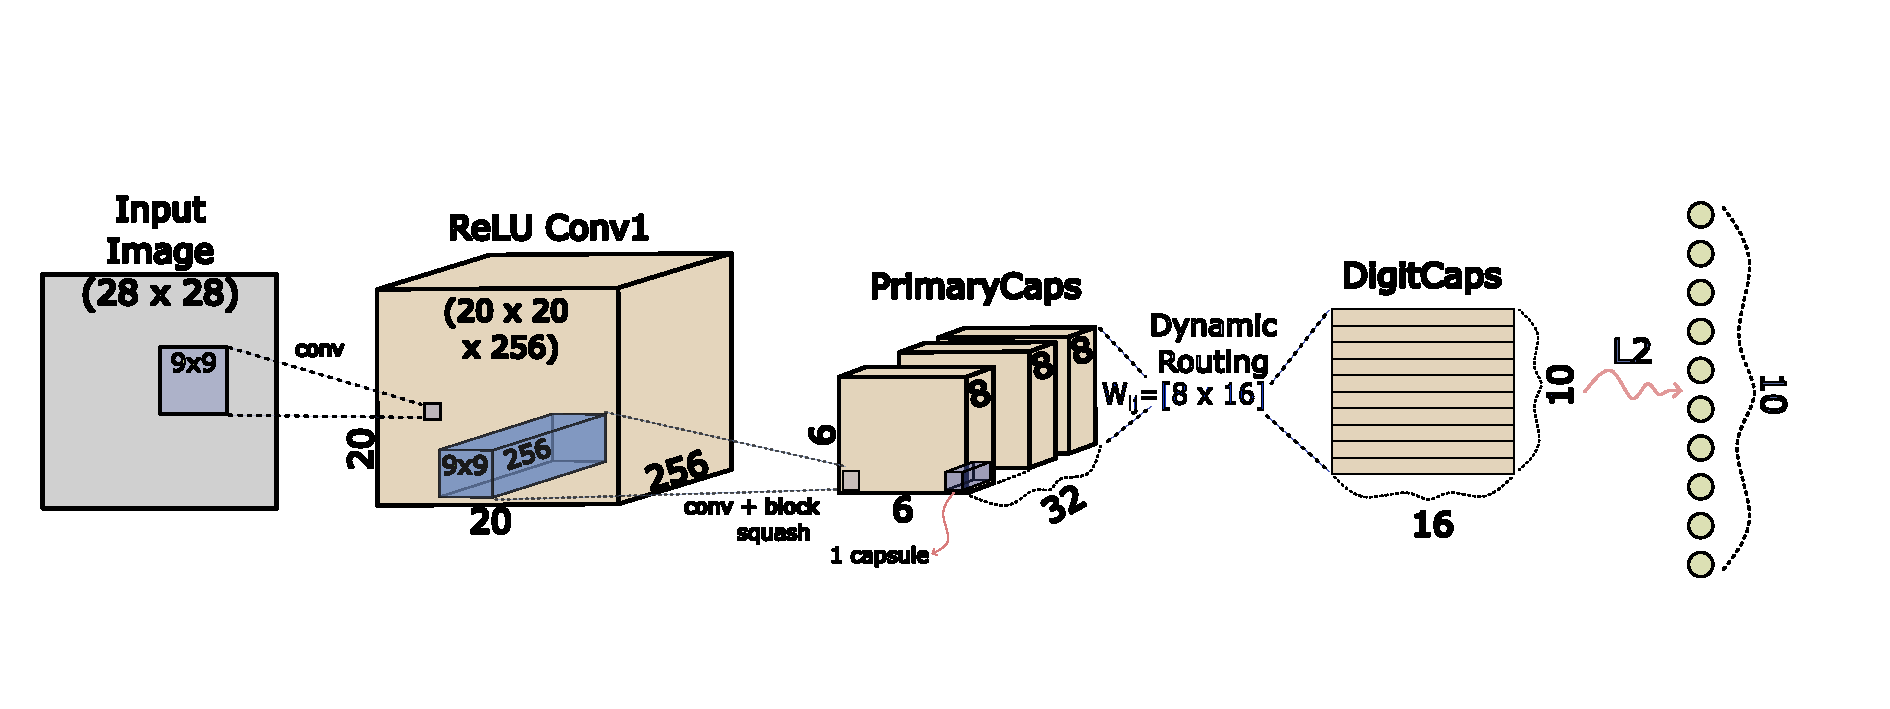
\includegraphics[width=0.95\textwidth]{images/chapter method/first_method_architecture_encoder.pdf}
    \caption{Η αρχιτεκτονική του νευρωνικού δικτύου με κάψουλες της πρώτης μεθόδου. \textit{Παράχθηκε από το \href{https://inkscape.org/}{\en{Inkscape}}}.}
    \label{fig:method_1_architecture}
  \end{figure}

Το βασικό μοντέλο που χρησιμοποιείται στην πλειοψηφία των πειραμάτων μας παρουσιάζεται στο σχήμα \ref{fig:method_1_architecture}. Αποτελείται από 3 επίπεδα εκ των οποίων τα πρώτα δύο είναι συνελικτικά (ονόματι \en{Conv1} και \en{PrimaryCaps}) και το τρίτο πλήρως διασυνδεδεμένο (επίπεδο \en{DigitCaps}). Πιο αναλυτικά, το επίπεδο \en{Conv1} έχει 256 πυρήνες συνέλιξης μεγέθους $9 \times 9$, βήμα (\en{stride}) ίσο με 1 και συνάρτηση ενεργοποίησης \en{ReLU}.\par

Αναφορικά με το επίπεδο \en{PrimaryCaps}, ο ρόλος του είναι αυτός των ανάστροφων γραφικών, όπως εξηγήσαμε στην ενότητα \ref{sec:capsule_theory}. Πρακτικά, αποτελεί ένα συνελικτικό επίπεδο με 32 κανάλια από 8\en{D} κάψουλες\textendash διανύσματα. Δηλαδή, κάθε κάψουλα περιέχει 8 μονάδες συνέλιξης με πυρήνες μεγέθους $9 \times 9$ και βήμα 2. Κατά αυτόν τον τρόπο, κάθε κάψουλα \textquote{βλέπει} $256 \times 9 \times 9$ στοιχεία (μονάδες) από τους χάρτες χαρακτηριστικών του προηγούμενου επιπέδου.\par

Όπως φαίνεται και από το σχετικό σχήμα, με αυτό το επίπεδο σχηματίζεται ένα πλέγμα από $32 \times 6 \times 6$ κάψουλες. Να σημειώσουμε ότι επειδή το επίπεδο \en{PrimaryCaps} αποτελεί ένα συνελικτικό επίπεδο από κάψουλες, τα βάρη των πυρήνων (κυλιόμενων παραθύρων) σε κάθε πλαίσιο στους άξονες $x-y$ $6 \times 6$ διαμοιράζονται. Η ειδοποιός διαφορά με ένα συνελικτικό επίπεδο χωρίς κάψουλες είναι στην συνάρτηση ενεργοποίησης. Αυτή αφενός είναι μια συνάρτηση σύνθλιψης (\en{squashing function}) που θα ορίσουμε στη συνέχεια και αφετέρου εφαρμόζεται σε ομάδες 8 στοιχείων τη φορά (δηλαδή σε κάθε 8\en{D} κάψουλα). Συνεπώς, το επίπεδο \en{PrimaryCaps} μπορεί να θεωρηθεί ως απλό συνελικτικό επίπεδο με $32 \times 8$ κανάλια στο οποίο, ανά ομάδες των 8 στοιχείων στη διάσταση βάθους, εφαρμόζεται μη γραμμικότητα τύπου \textquote{μπλοκ} (\en{block non\textendash linearity}).\par

Το τελευταίο επίπεδο είναι το \en{DigitCaps} το οποίο έχει σαν έξοδο (συνήθως 10 από) 16\en{D} κάψουλες\textendash διανύσματα των οποίων το μήκος ($L_2$ νόρμα), όπως έχουμε προαναφέρει, χρησιμοποιείται για τον εντοπισμό της κλάσης πρόβλεψης. Ανάμεσα στα πλήρως διασυνδεδεμένα επίπεδα \en{PrimaryCaps} και \en{DigitCaps} λαμβάνει χώρα ο αλγόριθμος δρομολόγησης μέσω συμφωνίας που αναλύουμε παρακάτω. Όπως φαίνεται και από το σχήμα, μεταξύ των δύο επιπέδων παρεμβάλλονται και μια σειρά από πίνακες βαρών ($6\times 6 \times 32 \times 10$ τέτοιοι πίνακες διάστασης $8 \times 16$) που μετασχηματίζουν τις τιμές της κάθε 8\en{D} κάψουλας του επιπέδου \en{PrimaryCaps} σε 16\en{D} ψήφους, μια για κάθε κάψουλα γονέα (άρα 10 ψήφοι αντιστοιχούν σε κάθε κάψουλα επιπέδου \en{PrimaryCaps}). Επισημαίνουμε ότι οι πίνακες βαρών τροποποιούνται κατά την εκπαίδευση και δεν εξαρτώνται από το εκάστοτε μεμονωμένο παράδειγμα (αποθηκεύουν πληροφορία μεταξύ μερών \textendash όλου που είναι ανεξάρτητη από την οπτική γωνία).\par

\subsubsection{Ανακατασκευή}
\begin{figure}[h]
    \centering
    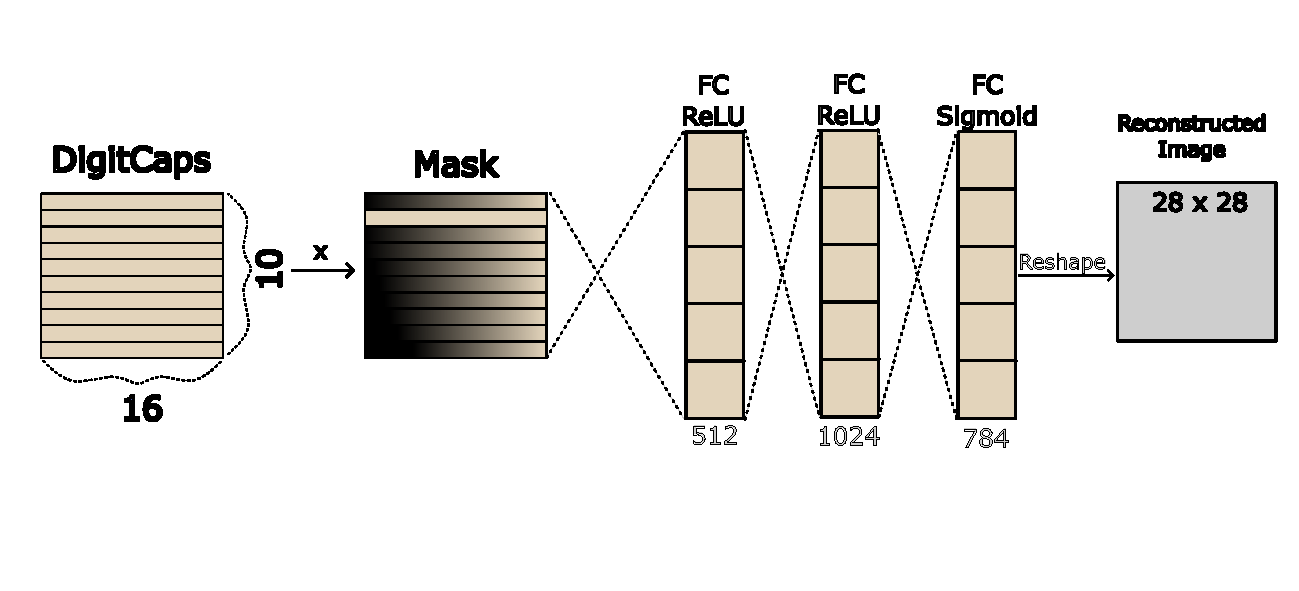
\includegraphics[width=0.95\textwidth]{images/chapter method/first_method_decoder.pdf}
    \caption{Η αρχιτεκτονική του αποκωδικοποιητή που διευκολύνει την εκπαίδευση του νευρωνικού δικτύου με κάψουλες. \textit{Παράχθηκε από το \href{https://inkscape.org/}{\en{Inkscape}}}.}
    \label{fig:method_1_decoder_architecture}
  \end{figure}

Προκειμένου να ενθαρρυνθεί η σύλληψη των παραμέτρων στιγμιότυπου του κάθε ψηφίου από το αντίστοιχο διάνυσμα \en{DigitCaps} χρησιμοποιείται ένας αποκωδικοποιητής του σχήματος \ref{fig:method_1_decoder_architecture}. Αυτός δομείται από 3 πλήρως διασυνδεδεμένα επίπεδα με αριθμό νευρώνων $160 \times 512, 512\times 1024$ και $ 1024 \times 28 \times 28 $ αντίστοιχα. Να σημειώσουμε ότι μεταξύ του επιπέδου \en{DigitCaps} και του πρώτου πλήρως διασυνδεδεμένου επιπέδου του αποκωδικοποιητή παρεμβάλλεται μια μάσκα που σκοπό έχει να μηδενίσει όλες τις κάψουλες εξόδου παρά αυτήν που σχετίζεται με το ψηφίο\textendash στόχο (\en{target}) κατά τη διάρκεια εκπαίδευσης ή αυτή που έχει το μεγαλύτερο μήκος κατά τη διάρκεια ελέγχου. \footnote{Όπως έχει γίνει σαφές, ο αύξοντας αριθμός της κάψουλας με τη μεγαλύτερη $\mathcal{L}_2$ νόρμα (μήκος) είναι και η κλάση πρόβλεψης $\hat{y}$.} Έτσι, ο αποκωδικοποιητής δέχεται σαν είσοδο μόνο ένα διάνυσμα (\en{DigitCap}) και έχει ως έξοδο μια εικόνα $28 \times 28$ που μέσω εκπαίδευσης επιδιώκεται να είναι όσο πιο πιστό αντίγραφο γίνεται της εικόνας εισόδου.\par

\subsection{Συνάρτηση Σύνθλιψης}

Όπως έχουμε αναφέρει, τόσο για τον υπολογισμό των \en{PrimaryCaps} όσο και για τον υπολογισμό των \en{DigitCaps} μέσω του αλγορίθμου δρομολόγησης, χρησιμοποιείται η συνάρτηση σύνθλιψης (\en{squashing function}). Πρόκειται για μια μη γραμμική συνάρτηση που δέχεται ένα διάνυσμα τυχαίου μήκους και εγγυάται ότι στην έξοδό της, το μήκος του διανύσματος θα ανήκει στο διάστημα $(0,1)$. Με αυτόν τον τρόπο, το μήκος του διανύσματος μοντελοποιεί την πιθανότητα ενεργοποίησης της εκάστοτε κάψουλας.\par

Με μαθηματικούς όρους, έχουμε:
\begin{equation}
    squash(x) = \frac{\left\lVert x\right\rVert^2}{1+\left\lVert x\right\rVert^2} \frac{x}{\left\lVert x\right\rVert}
\end{equation}

\subsection{Δυναμικός Αλγόριθμος Δρομολόγησης μέσω Συμφωνίας}

Ο αλγόριθμος μέσω συμφωνίας λαμβάνει χώρα μεταξύ δύο επιπέδων από κάψουλες και όπως έχουμε εξηγήσει αναλαμβάνει τον ρόλο της ανάθεσης μερών των αντικειμένων σε ένα από τα αντικείμενα στόχους. Πιο αναλυτικά, η διαδικασία που λαμβάνει χώρα για τον σχηματισμό των καψουλών γονέων από τις κάψουλες παιδιά είναι η εξής:
\begin{enumerate}
    \item Από την κάθε μια κάψουλα παιδί (έστω $u_i$) παράγονται τόσοι ψήφοι ($\hat{u}_{j|i}$) όσες και οι κάψουλες γονείς. Οι ψήφοι αποτελούν προβλέψεις της πόζας της εκάστοτε κάψουλας γονέα και υπολογίζονται πολλαπλασιάζοντας την κάψουλα παιδί με τον πίνακα βαρών $W_{ij}$ που συνδέει το τμήμα του αντικειμένου $i$ με την οντότητα που αναπαριστά η κάψουλα $j$. Έτσι έχουμε: 
    \begin{equation}
    \hat{u}_{j|i} = W_{ij} u_i
    \end{equation}
    \item Μέσω του αλγορίθμου δρομολόγησης που θα εξετάσουμε στη συνέχεια, υπολογίζονται τα διανύσματα των καψουλών γονέων ($s_j$) ως σταθμισμένα αθροίσματα των ψήφων παιδιών, δηλαδή:
    \begin{equation}
    s_j = \sum_i c_{ij} \hat{u}_{j|i}
    \end{equation}
    όπου τα $c_{ij}$ είναι οι παράμετροι σύζευξης (\en{coupling coefficients}). Αυτές υπολογίζονται σύμφωνα με τη συνάρτηση \en{softmax}, δηλαδή:
    \begin{equation}
    c_{ij} = \frac{exp(b_{ij})}{\sum_k exp(b_{ik})}
    \end{equation}
    ανάλογα με τα $b_{ij}$ (\en{log priors}) που τροποποιούνται σε κάθε επανάληψη του αλγορίθμου.
\end{enumerate}

Πλέον, είμαστε σε θέση να παρουσιάσουμε τον δυναμικό αλγόριθμο δρομολόγησης μέσω συμφωνίας αναλυτικά. Αυτός, όπως έχει γίνει σαφές, λαμβάνει μέρος αμέσως μετά τον υπολογισμό των ψήφων.

\algnewcommand{\Initialize_gr}[1]{%
  \State \textbf{\gr{Αρχικοποίηση:}}
  \State \hspace{\algorithmicindent }\parbox[t]{.8\linewidth}{\raggedright #1}
}

\algnewcommand{\Initializee}[1]{%
  \State \textbf{Initialize:}
  \State \hspace{\algorithmicindent }\parbox[t]{.8\linewidth}{\raggedright #1}
}

\en{
\begin{algorithm}[H]
    \caption{\gr{Δυναμικός Αλγόριθμος Δρομολόγησης μέσω Συμφωνίας}}\label{alg:dynam_routing}
    \begin{algorithmic}[1]
        \Function{Routing}{$\hat{u}_{j|i}, r, l$}
        \Initialize_gr{$\forall$ \gr{κάψουλα} $i$ $\in$ \gr{επίπεδο} $l$ \gr{και κάψουλα} $j \in$ \gr{επίπεδο} $(l+1)$: $b_{ij} \gets 0$}
            \For{$r$ \gr{επαναλήψεις}}
            \State $\forall$ \gr{κάψουλα} $i$ $\in$ \gr{επίπεδο} $l$: $c_i \gets softmax(b_i)$
            \State $\forall$ \gr{κάψουλα} $j$ $\in$ \gr{επίπεδο} $(l+1)$: $s_j \gets \sum_i c_{ij}\hat{u}_{j|i}$
            \State $\forall$ \gr{κάψουλα} $j$ $\in$ \gr{επίπεδο} $(l+1)$: $v_j \gets squash(s_j)$
            \State $\forall$ \gr{κάψουλα} $i$ $\in$ \gr{επίπεδο} $l$ \gr{και} \gr{κάψουλα} $j$ $\in$ \gr{επίπεδο} $(l+1)$: $b_{ij} \gets b_{ij} + \hat{u}_{j|i} \times v_j$
            \EndFor
            \State \Return $v_j$
        \EndFunction
    \end{algorithmic}
    \end{algorithm}
}

\subsubsection{Μερικές Σημειώσεις Σχετικά με τον Αλγόριθμο Δρομολόγησης}

Προκειμένου να διευκολύνουμε τον αναγνώστη στη διαισθητική κατανόηση αλλά και πρακτική υλοποίηση του αλγορίθμου \ref{alg:dynam_routing} κάνουμε τις εξής παρατηρήσεις:
\begin{itemize}
    \item Σε κάθε κάψουλα γονέα (\en{DigitCaps}) αντιστοιχούν τόσες ψήφοι όσες είναι και οι κάψουλες παιδιά (\en{PrimaryCaps}). Επειδή κάθε ψήφος παράγεται από έναν μοναδικό πίνακα βαρών $W_{ij}$, γίνεται αντιληπτό ότι κάθε γονέας \textquote{βλέπει} διαφορετικές ψήφους.
    \item Αρχικοποιώντας τα $b_{ij}$ με την τιμή $0$, στην πρώτη επανάληψη του αλγορίθμου δρομολόγησης διαμορφώνονται τα διανύσματα των καψουλών γονέων ($s_j$) ως οι μέσοι όροι των ψήφων που τους αντιστοιχούν.
    \item Σε κάθε επανάληψη, κάθε κάψουλα παιδί $i$ τροποποιεί τα βάρη δρομολόγησής της (\en{coupling coefficients}) $c_{ij}$ ανάλογα με το πόσο συμφωνεί η πρόβλεψή του ($\hat{u}_{j|i}$) με το διάνυσμα $s_j$ της κάθε κάψουλας γονέα. Η συμφωνία αυτή εκτιμάται με τη χρήση του εσωτερικού γινομένου $\hat{u}_{j|i} \times v_j$.
    \item Όταν το διάνυσμα πρόβλεψης $\hat{u}_{j|i}$ παρουσιάζει μεγάλη συμφωνία με το διάνυσμα $s_j$, η ποσότητα $c_{ij}$ θα αυξηθεί, προκαλώντας (πιθανότατα) ακόμα μεγαλύτερη συμφωνία στην επόμενη επανάληψη. Αναπόφευκτα, λόγω του περιορισμού $\sum_j c_{ij} = 1$, αν μια κάψουλα γονέας (έστω $k$) παρουσιάζει μικρή συμφωνία με την αντίσοιχη πρόβλεψη $\hat{u}_{k|i}$ της κάψουλας $i$, η ποσότητα $c_{ik}$ θα μειωθεί. Συνεπώς, η συγκεκριμένη κάψουλα παιδί $i$ θα έχει μικρό ποσοστό στο μερίδιο διαμόρφωσης του διανύσματος $s_k$.
    \item Κάψουλες για τις οποίες πολλές ψήφοι συμφωνούν καταλήγουν μετά από λίγες επαναλήψεις του αλγορίθμου δρομολόγησης (συνήθως 3) να έχουν διανύσματα με μεγάλο μήκος (και άρα μεγάλη πιθανότητα). Αντίθετα, κάψουλες γονείς που έχουν μικρή συμφωνία με τις προβλέψεις των παιδιών, λαμβάνουν μικρά σε μήκος διανύσματα (λόγω των μικρών $c_{ij}$) που αντικρούουν το ένα το άλλο (\en{cancel each other out}) κατά την πράξη του σταθμισμένου αθροίσματος.
    \item Πρακτικά, επειδή η κάθε κάψουλα γονέα $j$ διαμορφώνεται από τις αντίστοιχες ψήφους των καψουλών παιδιών, μεγάλη συμφωνία μεταξύ αυτών προκύπτει από μεγάλη συμφωνία των παιδιών στον χώρο των ψήφων (για τον γονέα $j$). Με άλλα λόγια, η ύπαρξη μιας πυκνής συστάδας (\en{cluster}) από ψήφους για την πόζα ενός γονέα $j$ συνεπάγεται ότι το διάνυσμά του γονέα $s_j$ θα έχει μεγάλο μέτρο\footnote{Με εξαίρεση αν, λόγω ανταγωνισμού, υπάρχουν πολλές, πυκνότερες συστάδες που αντιστοιχούν σε άλλες κάψουλες γονείς.}. Με αυτήν την παρατήρηση, ο όρος \textquote{φιλτραρίσματος μέσω της πολυδιάστατης σύμπτωσης} (\en{high dimensional coincidence filtering}) γίνεται πλήρως κατανοητός.
\end{itemize}


\subsection{Συνάρτηση Σφάλματος}

Για την εκπαίδευση του νευρωνικού δικτύου με κάψουλες εισάγεται η συνάρτηση \textquote{Απώλειας Περιθωρίου} (\en{Margin Loss}). Μέσω αυτής της συνάρτησης, κατά την εκπαίδευση ενθαρρύνεται η προσαρμογή των βαρών του δικτύου ώστε το διάνυσμα \en{DigitCap} που αναπαριστά την εκάστοτε κλάση πρόβλεψης $\hat{y}$ να έχει μεγάλο μήκος ενώ τα άλλα διανύσματα που αντιστοιχούν στις υπόλοιπες κλάσεις που δεν εντοπίζονται στην εικόνα εισόδου να έχουν (σχεδόν) μηδενικό μήκος. Επιπλέον, επιτρέπει την εκπαίδευση σε περιπτώσεις όπου στην εικόνα εισόδου απαντώνται περισσότερα του ενός αντικείμενα που ανήκουν σε διαφορετικές κλάσεις. Αναλυτικότερα, η συνάρτηση σφάλματος ορίζεται ξεχωριστά για κάθε κάψουλα \en{DigitCap} $k$ ως εξής:
\begin{equation}
    L_k = T_k max(0, m^+ - \left\lVert v_k\right\rVert)^2 + \lambda (1-T_k) max(0, \left\lVert v_k\right\rVert - m^-)^2
\end{equation}
όπου $T_k = 1$ αν και μόνο αν το αντικείμενο κλάσης $k$ βρίσκεται στην εικόνα εισόδου. Επίσης, συνήθως είναι $m^+ = 0.9$ και $m^- = 0.1$ ενώ η τιμή της παραμέτρου λ είναι $\lambda = 0.5$. Η συνάρτηση σφάλματος προκύπτει ως: \begin{equation}
  \mathcal{L} = \sum_k L_k.
\end{equation}

Σε περίπτωση που χρησιμοποιείται και το πλήρως διασυνδεδεμένο δίκτυο αποκωδικοποιητή που έχει ως έξοδο προβλέψεις (σε μορφή διανύσματος) $\hat{x}$ τότε έχουμε: 
\begin{equation}
\mathcal{L} = \sum_k L_k + \lambda_{rec} \left\lVert x - \hat{x}\right\rVert^2 
\end{equation}
όπου $\lambda_{rec} = 0.0005$ ο όρος που μειώνει τη βαρύτητα του σφάλματος ανακατασκευής.


\section{\en{Matrix Capsules with EM Routing}}

Η μέθοδος αυτή χρησιμοποιείται σε ορισμένα πειράματα της διπλωματικής προκειμένου να δοκιμαστεί αν ορισμένες βασικές υποθέσεις των νευρωνικών δικτύων με κάψουλες διατηρούνται στη νεότερη υλοποίηση της τεχνολογίας από την ομάδα του \en{G. Hinton}. Αν και οι δύο αρχικές μέθοδοι που περιγράφουμε δε διαφέρουν στη θεωρία που έχουμε περιγράψει, η πιο καινούρια υλοποίηση παρουσιάζει τεχνικές βελτιώσεις με τις οποίες επιτυγχάνεται αυξημένη ακρίβεια στα πειραματικά αποτελέσματα. Οι πιο βασικές από αυτές τις βελτιώσεις είναι οι εξής:
\begin{itemize}
  \item Η αντικατάσταση του δυναμικού αλγορίθμου δρομολόγησης με τον αλγόριθμο δρομολόγησης βασισμένο στη μεγιστοποίηση προσδοκιών (\en{EM}). Κατά τη δρομολόγηση των ψήφων του ενός επιπέδου ($l$) στις κάψουλες του επόμενου ($l=1$), κάθε κάψουλα γονέας μοντελοποιείται σαν μια Γκαουσιανή κατανομή (με $\mu \in \Re^{16} και \sigma \in \Re^{16}$) που προσαρμόζεται επαναλληπτικά για να \textquote{εξηγήσει} τις ψήφους\textendash σημεία (\en{datapoints}).
  \item Η αλλαγή του τρόπου αναπαράστασης της κάψουλας η οποία τώρα επιτελείται χρησιμοποιώντας έναν πίνακα $4\times 4$ για την πόζα $M_i$ και μια ξεχωριστή λογιστική μονάδα (\en{logistic unit}) $\alpha_i$ για την πιθανότητα ύπαρξης της, συνυφασμένης με την κάψουλα, οντότητας. Όπως είναι λογικό, οι ψήφοι $V_{ij}$ και πάλι προκύπτουν ως εξής: $V_{ij} = M_iW_{ij}, W_{ij} \in \Re^{4\times 4}$.
\end{itemize}

Δυστυχώς, η δημοσίευση του έργου \cite{hinton2018matrix} δε συνοδεύτηκε από κώδικα. Πολλοί ερευνητές επιδίωξαν να δημοσιεύσουν τη δική τους υλοποίηση αλλά τα πειραματικά αποτελέσματα ήταν πολύ πιο χαμηλά από αυτά που αναφέρονται στο σχετικό έργο. Η καλύτερη, ανοιχτού κώδικα υλοποίηση που εντοπίσαμε ακούει στο όνομα \en{Avoiding Implementation Pitfalls of "Matrix Capsules with EM Routing by Hinton et al."} \cite{gritzman2019avoiding}. Στην παρούσα διπλωματική εργασία, ακολουθούμε αυτήν την υλοποίηση (με μικρές αλλαγές) καθώς φαίνεται να είναι η πιο πιστή και επιτυχημένη υλοποίηση του δικτύου που περιγράφεται στο βασικό έργο. Μάλιστα, επιτυγχάνει ακρίβεια αποτελεσμάτων που είναι πολύ κοντά σε αυτήν που αναγράφεται στο \cite{hinton2018matrix}.\par

Σε αυτή την ενότητα, πρώτα θα παρουσιάσουμε την αρχιτεκτονική του νευρωνικού δικτύου με κάψουλες. Έπειτα θα παραθέσουμε τον νέο αλγόριθμο δρομολόγησης με συμφωνία μαζί με ορισμένες παρατηρήσεις. Τέλος, θα αναφερθούμε σε μερικές λεπτομέρειες υλοποίησης που αφορούν κυρίως τη διαδικασία δρομολόγησης μεταξύ διαδοχικών συνελικτικών επιπέδων από κάψουλες. Για περισσότερες λεπτομέρειες υλοποίησης, παραπέμπουμε τον αναγνώστη για άλλη μια φορά στην ιστοσελίδα όπου είναι αναρτημένος ο κώδικάς μας.

\subsection{Αρχιτεκτονική Νευρωνικού Δικτύου}

\begin{figure}[h]
  \centering
  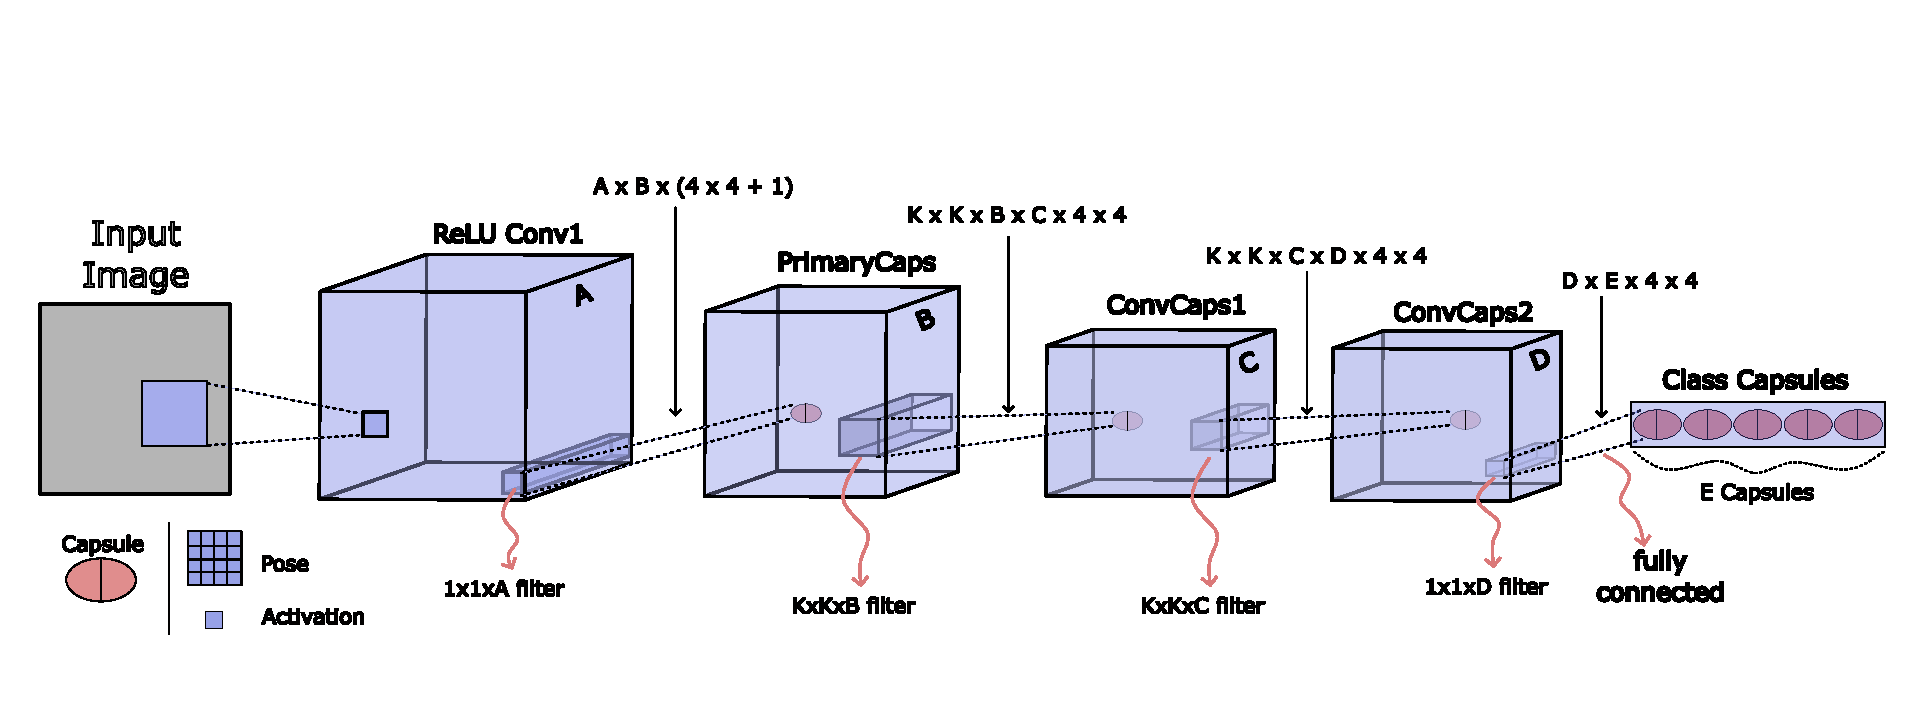
\includegraphics[width=0.95\textwidth]{images/chapter method/second_method_architecxture.pdf}
  \caption{Η αρχιτεκτονική του νευρωνικού δικτύου με κάψουλες της δεύτερης μεθόδου. \textit{Παράχθηκε από το \href{https://inkscape.org/}{\en{Inkscape}}}.}
  \label{fig:method_2_architecture}
\end{figure}

Στο σχήμα \ref{fig:method_2_architecture} παρατηρούμε τη γενική αρχιτεκτονική που χρησιμοποιείται σε αυτή τη μέθοδο. Κατά την περιγραφή της χρησιμοποιούμε τις μεταβλητές \en{A, B, C, D} για να αναφερθούμε σε παραμετροποιήσιμα χαρακτηριστικά του δικτύου. Όπως παρατηρούμε, όλα τα επίπεδα είναι συνελικτικά με εξαίρεση το τελευταίο, πλήρως διασυνδεδεμένο επίπεδο ενώ επίσης όλα αποτελούν επίπεδα από κάψουλες με εξαίρεση το πρώτο.\par

Ξεκινώντας από το πρώτο, πρόκειται για ένα απλό συνελικτικό επίπεδο με κυλιόμενο παράθυρο $5 \times 5$, βήμα 2 και μη γραμμική συνάρτηση ενεργοποίησης \en{ReLU}. Το επίπεδο αυτό απαρτίζεται από \en{A} τέτοια κυλιόμενα παράθυρα με αποτέλεσμα να παράγονται \en{A} χάρτες χαρακτηριστικών. Η διάσταση των χαρτών χαρακτηριστικών εξαρτάται από το μέγεθος της εικόνας εισόδου και μπορεί να υπολογιστεί από τις σχέσεις \ref{eq:width_conv} και  \ref{eq:height_conv}.\par

Συνεχίζοντας την ανάλυση του σχήματος από αριστερά προς τα δεξιά έχουμε το πρώτο επίπεδο από κάψουλες (\en{PrimaryCaps}). Το βάθος του επιπέδου αυτού είναι \en{B}. Το χαρακτηριστικό αυτό το ονομάζουμε και αριθμό των τύπων καψουλών (\en{number of capsule types}) και κάθε τύπος κάψουλας αναπαριστά (άρρητα) μια συγκεκριμένη οντότητα\footnote{Κάψουλες ίδιου τύπου μαθαίνουν να αναγνωρίζουν την ίδια οντότητα αλλά σε διαφορετικές περιοχές της εικόνας.}. Το επίπεδο \en{PrimaryCaps} προκύπτει από τους προαναφερθέντες χάρτες χαρακτηριστικών έπειτα από συνέλιξη με πυρήνα $1 \times 1$ και βήμα 1. Πιο συγκεκριμένα, ο πίνακας πόζας μιας κάψουλας (\en{PrimaryCap}) προκύπτει από ένα σύνολο $ A \times 4 \times 4$ εκπαιδευόμενων (\en{learned}) βαρών που επενεργούν πάνω στο σημείο του επιπέδου \en{Conv1} που αντιστοιχεί στη συγκεκριμένη κάψουλα. Ουσιαστικά, κάθε πεδίο του $4 \times 4$ πίνακα προκύπτει ως γραμμικός συνδυασμός των \en{A} στοιχείων του επιπέδου \en{Conv1} (ένα από κάθε κανάλι) βεβαρημένων από \en{A} εκπαιδευόμενες παραμέτρους. Η τιμή ενεργοποίησης της κάψουλας προκύπτει με παρόμοιο τρόπο (δηλαδή αποτελεί το γραμμικό συνδυασμό των ίδιων \en{A} στοιχείων του \en{Conv1} με τα \en{A} βάρη) αλλά αυτή τη φορά, στο αποτέλεσμα εφαρμόζεται η σιγμοειδής συνάρτηση (ώστε το αποτέλεσμα να ανήκει στο διάστημα [0,1]). Σημειώνουμε ότι για κάθε τύπο κάψουλας (δηλαδή για καθένα από τα \en{B} κανάλια από κάψουλες) τα βάρη $ A \times (4 \times 4 + 1) $ διαμοιράζονται.\par

\begin{figure}[h]
  \centering
  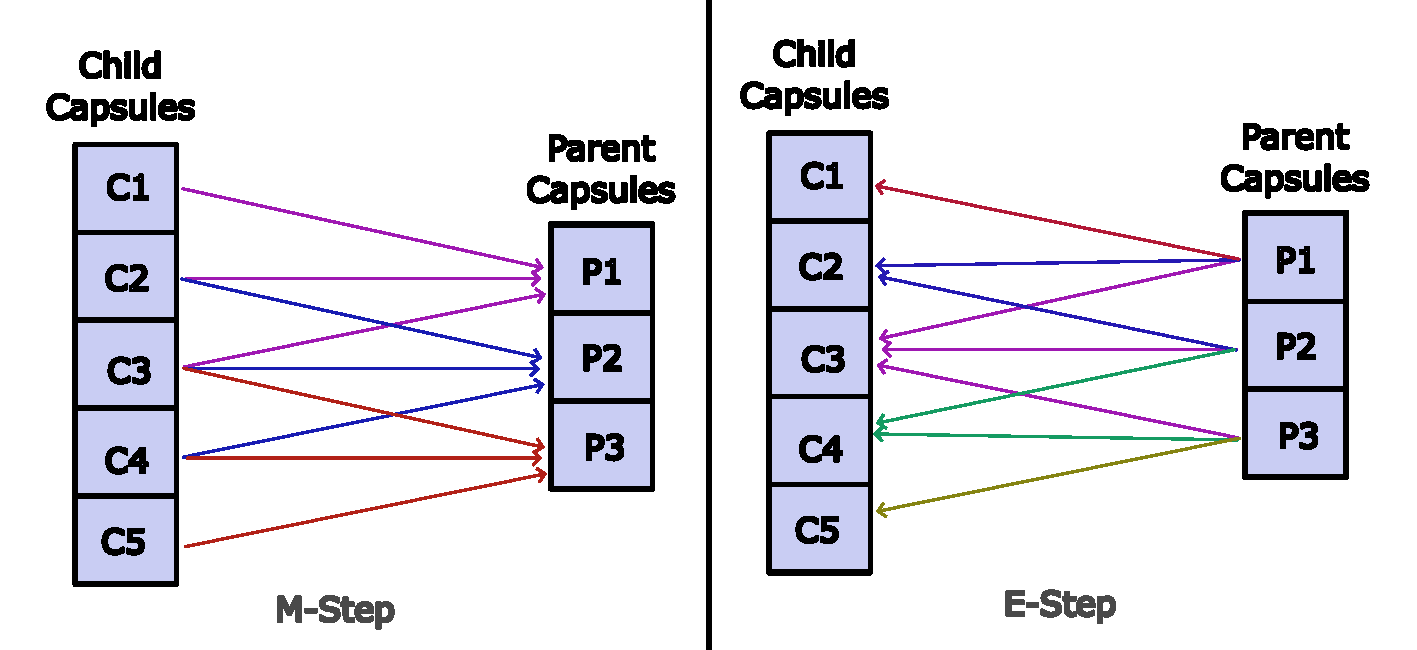
\includegraphics[width=0.95\textwidth]{images/chapter method/second_method_EM.pdf}
  \caption{Στο σχήμα παρατηρούμε τη διασύνδεση μεταξύ των καψουλών δύο διαδοχικών επιπέδων κατά τις φάσεις \en{M} και \en{E} του αλγορίθμου δρομολόγησης. Για λόγους απλότητας, απεικονίζεται η περίπτωση όπου έχουμε μονοδιάστατη συνέλιξη (\en{1D convolution}). \textit{Παράχθηκε από το \href{https://inkscape.org/}{\en{Inkscape}}}.}
  \label{fig:method_2_EM}
\end{figure}

Στη συνέχεια ακολουθούν τα επίπεδα \en{ConvCaps1} και \en{ConvCaps2}. Πρόκειται για δύο συνελικτικά επίπεδα από κάψουλες τα οποία έχουν \en{C} και \en{D} τύπους από κάψουλες, πυρήνες $3 \times 3$ και βήμα 2 και 1 αντίστοιχα. Ο σχηματισμός όμως των \en{ConvCaps1} και \en{ConvCaps2} δεν είναι προφανής. Πιο αναλυτικά, για τον σχηματισμό του καθενός τέτοιου επιπέδου λαμβάνει χώρα ο αλγόριθμος δρομολόγησης με συμφωνία βασιζόμενος στον \en{EM} που θα αναλύσουμε παρακάτω. Στο σημείο αυτό αξίζει να σημειωθεί ότι αντίθεση με δύο πλήρως διασυνδεδεμένα επίπεδα από κάψουλες, σε δύο συνελικτικά επίπεδα από κάψουλες οι γονείς (κάψουλες του επιπέδου $L + 1$) ανταγωνίζονται να διεκδικήσουν τις ψήφους των παιδιών (κάψουλες επιπέδου $L$) που ανήκουν σε μια γειτονιά ($K\times K = 3 \times 3$) του επιπέδου $L$ (κεντραρισμένη στην κάψουλα γονέα). Κατά αυτόν τον τρόπο, η εκάστοτε κάψουλα γονέας του επιπέδου $L + 1$ στέλνει ανατροφοδότηση (σύμφωνα με τον αλγόριθμο δρομολόγησης) μόνο στα παιδιά που ανήκουν στο οπτικό του πεδίο (βλ. σχήμα \ref{fig:method_2_EM}). Αντίστοιχα, τα παιδιά δεν παράγουν ψήφους για όλες τις κάψουλες του επόμενου επιπέδου αλλά μόνο για αυτές στων οποίων το οπτικό πεδίο ανήκουν. Επειδή μάλιστα οι πίνακες μετασχηματισμού $W_ij$ διαμοιράζονται στις χωρικές διαστάσεις $x-y$, για τον σχηματισμό του επιπέδου \en{ConvCaps1} απαιτούνται $K \times K \times B \times C \times 4 \times 4$ εκπαιδευόμενα (\en{learned}) βάρη (ανάλογα για το \en{ConvCaps2} απαιτούνται $K \times K \times C \times D \times 4 \times 4$). Αυτό το νούμερο προκύπτει λογικά αν αναλογιστεί κανείς ότι:
\begin{itemize}
  \item Ο κάθε πίνακας μετασχηματισμού έχει διάσταση $4 \times 4$. 
  \item Σε κάθε σημείο $i$ του πυρήνα (\en{kernel}) αντιστοιχεί ξεχωριστός πίνακας βαρών $Wij$, άρα έχουμε $K \times K$ τέτοιους πίνακες μεγέθους $4\times 4$.
  \item Το κυλιόμενο παράθυρο $K \times K$ έχει βάθος \en{B}, όσος και ο αριθμός των τύπων καψουλών εισόδου. Άρα είναι $B \times K \times K \times 4 \times 4$ βάρη.
  \item Θέλουμε \en{C} κανάλια εξόδου (ή αλλιώς τύπους από κάψουλες). Συνεπώς, έχουμε \en{C} κυλιόμενα παράθυρα.
\end{itemize}  

Το τελευταίο επίπεδο είναι το \en{Class Capsules} όπου κάθε κάψουλά του αντιστοιχεί σε μια κλάση. Η κάψουλα με τη μεγαλύτερη τιμή ενεργοποίησης (\en{logistic unit}) σηματοδοτεί την κλάση πρόβλεψης του νευρωνικού δικτύου όταν αυτό τροφοδοτείται με μια εικόνα ενός αντικειμένου. Τα περιεχόμενα των καψουλών στο τελευταίο επίπεδο σχηματίζονται με τον αλγόριθμο δρομολόγησης που παρουσιάζουμε παρακάτω. Επειδή τα δύο τελευταία επίπεδα είναι πλήρως διασυνδεδεμένα μεταξύ τους, κάθε κάψουλα του επιπέδου \en{ConvCaps2} παράγει μια ψήφο για κάθε κάψουλα του επιπέδου \en{Class Capsules}. Έτσι απαιτούνται $D \times E$ πίνακες μετασχηματισμού μεγέθους $4 \times 4$. Για να μη χαθεί η πληροφορία της θέσης (στον $x - y$ άξονα) στην οποία εντοπίζεται το κάθε αντικείμενο\textendash μέρος, μετά τον πολλαπλασιασμό της πόζας της κάθε κάψουλας με το κατάλληλο πίνακα μετασχηματισμού, στα πρώτα δύο κελιά της δεξιότερης στήλης του πίνακα ψήφου υπερτίθενται η γραμμή και η στήλη της κάψουλας από την οποία προήλθε (η ψήφος).\par

Όπως εξηγήσαμε, ακολουθούμε μια ελαφρός τροποποιημένη έκδοση της αρχιτεκτονικής που παρουσιάζεται στο \cite{hinton2018matrix} (βλ. πίνακα \ref{tab:method2_params_ABCD}). Η διαφορά έγκειται ότι η υλοποίηση που χρησιμοποιούμε (ακολουθώντας τις παρατηρήσεις και τον κώδικα του \cite{gritzman2019avoiding}) έχει συνήθως μικρότερο βάθος επιπέδων, χωρίς αυτό να είναι ο καθοριστικός παράγοντας της ελάχιστα χαμηλότερης απόδοσης που παρατηρείται όταν αντιπαραβάλλεται με τα αποτελέσματα της αυθεντικής υλοποίησης.
\begin{table}[h]
\begin{center}
  \begin{tabular}{| c | c c |} 
   \hline
   Παράμετρος & Αυθεντική Υλοποίηση & Απλοποιημένη \\ [0.5ex] 
   \hline\hline
   \en{A} & 32 & 64 \\ 
   \hline
   \en{B} & 32 & 8 \\
   \hline
   \en{C} & 32 & 16 \\
   \hline
   \en{D} & 32 & 16 \\ [1ex] 
   \hline
  \end{tabular}
  \caption{\label{tab:method2_params_ABCD}Πίνακας στον οποίο παρουσιάζεται η παραμετροποίηση της αρχιτεκτονικής όπως παρουσιάζεται στο έργο \cite{hinton2018matrix} (αυθεντική υλοποίηση) και όπως παρουσιάζεται στο \cite{gritzman2019avoiding} (απλοποιημένη). Η παράμετρος \en{E} είναι πάντα ίση με τον αριθμό των κλάσεων εξόδου.}
  \end{center}
\end{table}

\subsection{Υπολογισμός Τιμής Ενεργοποίησης}

Κατά αντιστοιχία με την προηγούμενη μέθοδο, οι κάψουλες παιδιά ψηφίζουν για το ποια εκτιμούν ότι είναι η πόζα του κάθε γονέα που \textquote{βλέπουν}. Σε αυτούς τους γονείς δρομολογούν τις ψήφους με βαρύτητα που υποδεικνύεται από τις πιθανότητες ανάθεσης (\en{assignment probabilities}) - συμβολίζονται με $R_{ij}$ και διαμορφώνονται δυναμικά από τον νέο αλγόριθμο δρομολόγησης. Προτού περιγράψουμε το νέο αλγόριθμο δρομολόγησης, κρίνεται σκόπιμο να εξηγήσουμε τον μηχανισμό με τον οποίο εκτιμάται αν θα ενεργοποιηθεί μια κάψουλα γονέας ή όχι (τιμή $\alpha_j$). Η λογική που ακολουθείται για τον σκοπό αυτό είναι εμπνευσμένη από την αρχή του ελαχίστου μήκους περιγραφής (\en{minimum description length principle}).\par

Πιο αναλυτικά, μέσα από τον αλγόριθμο δρομολόγησης που θα παρουσιάσουμε παρακάτω επιλέγεται κατά πόσον θα ενεργοποιηθεί ή όχι μια κάψουλα γονέας ανάλογα με το ποια κατάσταση ελαχιστοποιεί το κόστος περιγραφής\footnote{Φυσικά, η τιμή ενεργοποίησης $a_j$ λαμβάνει τιμές στο διάστημα [0,1] οπότε τυπικά υπάρχουν άπειρες ενδιάμεσες καταστάσεις.}. Για τον σχηματισμό του, λαμβάνονται υπόψη τα εξής:
\begin{itemize}
  \item Στην περίπτωση που δεν ενεργοποιηθεί μια κάψουλα γονέας, το κόστος προκύπτει από την τιμή $-\beta_u$ που πρέπει να \textquote{πληρώσουμε} για κάθε κάψουλα\textendash παιδί που αναθέτεται στον συγκεκριμένο γονέα (έστω $j$). Στη συνήθη περίπτωση που υπάρχει μερική ανάθεση μεταξύ παιδιού\textendash πατέρα ($R_{ij} \neq 1$), στο κόστος προστίθεται η ποσότητα $-\beta_u$ βεβαρημένη με το κλάσμα ανάθεσης $R_{ij}$. Συνεπώς, το κόστος για μια πλήρως απενεργοποιημένη κάψουλα $j$ θα είναι ίσο με:
  \begin{equation}
    -\beta_u \sum_i R_{ij}, \text{ όπου } i \in FoV(j) 
  \end{equation}
  \item Στην περίπτωση ενεργοποίησης της κάψουλας γονέα $j$ τότε \textquote{πληρώνουμε} πρώτα ένα κόστος $-\beta_{\alpha}$ που οφείλεται στην κωδικοποίηση των παραμέτρων που σχετίζονται με την κάψουλα γονέα. Επίσης, στο κόστος αυτό προστίθενται τα κόστη περιγραφής των διαφορών μεταξύ των ψήφων και της πόζας της κάψουλας $j$ στην οποία αναθέτονται (ζυγισμένα υπό τις πιθανότητες ανάθεσης). Η τελευταία ποσότητα μπορεί να προσεγγιστεί ως εξής:
  \begin{equation}
    cost_j = \sum_h cost_j^h = \sum_h \sum_i -R_{ij}ln(P^h_{i|j}),
  \end{equation} όπου ο δείκτης $h$ αναφέρεται στην $h$-οστή διάσταση του διανύσματος βάσης.
  Προς επεξήγηση της ανωτέρω σχέσης, να αναφέρουμε ότι ουσιαστικά, η ποσότητα $-R_{ij}ln(P^h_{i|j})$ περιγράφει το κόστος της διαφοράς της ψήφου $i$ και της πόζας της κάψουλας $j$ για τη διάσταση $h \in [1,4\times 4]$. Υπενθυμίζουμε, στο σημείο αυτό ότι οι ψήφοι $V_{ij} \in \Re^{4 \times 4}$ μοντελοποιούνται σαν σημεία στον χώρο $\Re^16$ και οι κάψουλες $M_j$ σαν Γκαουσιανές κατανομές με μέση τιμή $\mu_j \in \Re^{16}$ και διαγώνιο πίνακα συνδιακύμανσης $\varSigma$ με στοιχεία διαγωνίου που συγκροτούν το διάνυσμα $\sigma \in \Re^{16}$. Έτσι, μπορούμε να προσεγγίσουμε το κόστος για την περιγραφή ενός σημείου (ψήφου) $V_{ij}$ από την κατανομή (κάψουλα γονέας) $j$ ως την αρνητική, λογαριθμική, πολυμεταβλητή, γκαουσιανή πυκνότητα πιθανότητας (\en{negative log multivariate gaussian probability density}) παραμετροποιημένη από τα $\mu_j$ και $\sigma_j$ της κάψουλας $j$ υπολογισμένη στο σημείο της ψήφου $V_{ij}$ από την κάψουλα $i$ (φυσικά το κόστος θα είναι ζυγισμένο από την πιθανότητα ανάθεσης $R_{ij}$). Έτσι με μαθηματικούς όρους, η γκαουσιανή Σ.Π.Π. (\en{PDF}) υπολογισμένη στο σημείο $V_{ij}$ για τη διάσταση $h$ είναι:
  \begin{equation}
    P^h_{i|j} = \frac{1}{\sqrt{2\pi(\sigma_j^h)^2}}exp(-\frac{(V_{ij}^h-\mu_j^h)^2}{2(\sigma_j^h)^2}).
  \end{equation}
  Έτσι, ο αρνητικός λογάριθμος της ανωτέρω ποσότητας είναι:
  \begin{equation}
    -ln(P^h_{i|j}) = \frac{(V_{ij}^h-\mu_j^h)^2}{2(\sigma_j^h)^2} + ln(\sigma_j^h) + \frac{ln(2\pi)}{2}.
  \end{equation}
  Επανερχόμενοι στο συνολικό κόστος για τη διάσταση $h$, έχουμε:

  \begin{align}
    cost_j^h &= \sum_i - R_{ij} ln(P^h_{i|j}) \\ &= \frac{\sum_i R_{ij}(V_{ij}^h - \mu_j^h)^2}{2(\sigma_j^h)^2} + (ln(\sigma_j^h) + \frac{ln(2\pi)}{2})\sum_i R_{ij} \\ &= \frac{\sum_i R_{ij}(\sigma_j^h)^2}{2(\sigma_j^h)^2} + (ln(\sigma_j^h) + \frac{ln(2\pi)}{2})\sum_i R_{ij}  \\ &= (ln(\sigma_j^h) + \frac{1}{2} + \frac{ln(2\pi)}{2})\sum_i R_{ij} 
  \end{align}
\end{itemize}

Συνολικά λοιπόν, η συνάρτηση ενεργοποίησης της κάψουλας $j$ προκύπτει από την αντιπαραβολή του κόστους ενεργοποίησης και του κόστους απενεργοποίησής της. Τον ρόλο αυτό τον αναλαμβάνει η σιγμοειδής συνάρτηση (\en{sigmoid function}). Συνεπώς, έχουμε:
\begin{equation}
  \alpha_j = sigmoid(\lambda(\beta_{\alpha} - \beta_u \sum_i R_{ij} - \sum_h cost_j^h)).
\end{equation}
Το $\lambda$ είναι μια παράμετρος ανάστροφης θερμοκρασίας. Στην αρχή η παράμετρος είναι ίση με τη μονάδα και αυξάνεται σε κάθε επανάληψη του αλγορίθμου δρομολόγησης κάνοντας την κλίση της λογιστικής συνάρτησης μεγαλύτερη και ωθώντας τις τιμές ενεργοποίησης να λάβουν πιο ακραίες τιμές (0 ή 1). Αν ενσωματώσουμε στο $cost_j^h$ τον όρο $\beta_u \sum_i R_{ij}$ τότε έχουμε:
\begin{equation}
  \alpha_j = sigmoid(\lambda(\beta_{\alpha} - \sum_h \acute{cost}_j^h))
\end{equation}
όπου τώρα το κόστος είναι:
\begin{equation}
  \label{eq:cost_acute}
  \acute{cost} _j^h = (\beta_u + ln(\sigma_j^h) + const)\sum_i R_{ij}.
\end{equation}
Κλείνοντας την υποενότητα αυτή, να σημειώσουμε ότι οι ποσότητες $\beta_u$ και $\beta_{\alpha}$ μαθαίνονται κατά τη διάρκεια εκπαίδευσης του αλγορίθμου. Αυτός είναι και ένας λόγος για τον οποίο ο σταθερός όρος στη σχέση \ref{eq:cost_acute} μπορεί να παραληφθεί.

\subsection{Αλγόριθμος Δρομολόγησης \en{EM}}

Όπως έχουμε προαναφέρει, μεταξύ δύο διαδοχικών επιπέδων από κάψουλες λαμβάνει χώρα ο αλγόριθμος δρομολόγησης βασισμένο στη Μεγιστοποίηση Προσδοκειών (\en{Expectation Maximization}) μέσω του οποίου οι τιμές ενεργοποίησης και οι πόζες των καψουλών γονέων υπολογίζονται επαναληπτικά. Κατά αντιστοιχία με τον αυθεντικό αλγόριθμο \en{EM}, η επαναληπτική διαδικασία αποτελείται από δύο βήματα τα οποία εναλλάσσονται διαδεχόμενα το ένα το άλλο. Στο βήμα \en{E} υπολογίζονται οι πιθανότητες ανάθεσης $R_{ij}$ για κάθε ζευγάρι από κάψουλες μεταξύ των δύο επιπέδων. Ο υπολογισμός γίνεται χρησιμοποιώντας τις μέσες τιμές, τις διακυμάνσεις και τις τιμές ενεργοποίησης των καψουλών γονέων. Στο βήμα \en{M} υπολογίζονται οι παράμετροι των Γκαουσιανών κατανομών (που μοντελοποιούν τις κάψουλες γονείς) με βάση τα ανανεωμένα $R_{ij}$. Έτσι, μετά από ορισμένο αριθμό επαναλήψεων, ο αλγόριθμος συγκλίνει με αποτέλεσμα οι ενεργές κάψουλες γονείς να λαμβάνουν και να περιγράφουν συστάδες από όμοιες ψήφους παιδιών. \par

Μια περισσότερο τυπική περιγραφή του αλγορίθμου δρομολόγησης παρατίθεται παρακάτω. Σημειώνουμε ότι με $\Omega_L$ συμβολίζουμε το σύνολο όλων των καψουλών επιπέδου $L$. Επίσης, για τη διάσταση $H$ του πίνακα πόζας όταν αναδιατάσσεται σε διάνυσμα ισχύει ότι $Η = 16$.

\en{
\begin{algorithm}[H]
  \caption{\gr{Αλγόριθμος Δρομολόγησης Βασισμένος στον} \en{EM}}\label{alg:em_routing}
  \begin{algorithmic}[1]
      \Procedure{EM Routing}{$\alpha, V$}
      \Initialize_gr{$\forall$ $i$ $\in$ $\Omega_L$, $j \in \Omega_{L+1}: R_{ij} \gets 1/\left\lvert \Omega_{L+1}\right\rvert $
      }
      \For{$t$ \gr{επαναλήψεις}}
      \State $\forall j \in \Omega_{L+1}: M-Step(\alpha, R, V, j)$
      \State $\forall i \in \Omega_{L}: E-Step(\mu, \sigma, \alpha, V, i)$
      \EndFor
      \EndProcedure
      \Procedure{M-Step}{$\alpha, R, V, j$} \Comment{\gr{Για μια κάψουλα υψηλότερου επιπέδου, $j$}}
        \State $\forall i \in \Omega_L: R_{ij} \gets R_{ij} \ast \alpha_i$
        \State $\forall h: \mu_j^h \gets \frac{\sum_i R_{ij}V_{ij}^h}{\sum_i R_{ij}}$
        \State $\forall h: (\sigma_j^h)^2 \gets \frac{\sum_i R_{ij}(V_{ij}^h - \mu_j^h)^2}{\sum_i R_{ij}}$
        \State $\forall h: \acute{cost}^h \gets (\beta_u + log(\sigma_j^h)) \sum_i R_{ij}$ \label{op:sum_rij}
        \State $\alpha_j \gets logistic(\lambda(\beta_{\alpha} - \sum_h \acute{cost}^h))$ 
      \EndProcedure
      \Procedure{E-Step}{$\mu, \sigma, \alpha, V, i$} \Comment{\gr{Για μια κάψουλα χαμηλότερου επιπέδου, $i$}}
      \State $\forall j \in \Omega_{L+1}: p_j \gets \frac{1}{\sqrt{\prod _h^H 2\pi(\sigma_j^h)^2}} \exp(- \sum_h^H \frac{(V_{ij}^h - \mu_j^h)^2}{2(\sigma_j^h)^2})$
      \State $\forall j \in \Omega_{L+1}: R_{ij} \gets \frac{\alpha_j p_j}{\sum_{k \in \Omega_{L+1}} \alpha_k p_k}$
      \EndProcedure
  \end{algorithmic}
  \end{algorithm}
}

Για τον αλγόριθμο δρομολόγησης βασισμένο στον \en{EM} μπορούμε να κάνουμε τις εξής σημειώσεις:
\begin{itemize}
  \item Αρχικοποιούμε με ομοιόμορφο τρόπο τις πιθανότητες ανάθεσης $R_{ij}$ ώστε κάθε παιδί να συνδέεται ισοδύναμα με τους γονείς που ψηφίζει. Έπειτα, καλούμε (επαναληπτικά) το βήμα \en{M} και το βήμα \en{E}.
  \item Στο βήμα \en{M} υπολογίζουμε τα $\mu_j$ τα $\sigma_j$ και τα $\alpha_j$ βασιζόμενοι στα $R_{ij}, V_{ij}$ και εμμέσως, στις πιθανότητες ενεργοποίησης των παιδιών $\alpha_i$. Ουσιαστικά, στο βήμα αυτό υπολογίζεται ένα βελτιωμένο γκαουσιανό μοντέλο για την κάθε κάψουλα, μαζί με την πιθανότητα ανάθεσής της. 
  \item Στο βήμα \en{E} υπολογίζονται οι πιθανότητες μέλους (\en{membership probabilities}) $p_j$ που δείχνουν την πιθανότητα το \textquote{δείγμα} $i$ να ανήκει στην γκαουσιανή $j$. Επίσης, επανεκτημούνται οι πιθανότητες ανάθεσης $R_{ij}$. οι εν λόγω υπολογισμοί γίνονται χρησιμοποιώντας τις νέες κατανομές προέκυψαν από το βήμα \en{M}.
  \item Στο βήμα \ref{op:sum_rij} του αλγορίθμου (σχέση \ref{eq:cost_acute}) πρακτικά κλιμακώνουμε το κόστος ανάλογα με τη μέση ποσότητα δεδομένων που δέχονται οι κάψουλες γονείς στο εκάστοτε επίπεδο. Η ποσότητα αυτή υπολογίζεται από τον τύπο:
  \begin{equation}
    mean\_data = \frac{child_W \times child_H \times child_{CH}}{parent_W \times parent_H \times parent_{CH}},
  \end{equation}
  όπου $W, H$ και $CH$ δηλώνουν το πλάτος, το ύψος και το βάθος (αριθμός από τύπους) του επιπέδου από κάψουλες. \footnote{Η κλιμάκωση μπορεί να γίνει με διαίρεση του κόστους με τη μέση ποσότητα δεδομένων. Για περισσότερες πληροφορίες, παραπέμπουμε τον αναγνώστη στο \cite{gritzman2019avoiding}.}
  \item Μετά από δύο ή τρεις επαναλήψεις συνήθως, ο αλγόριθμος τερματίζει όπου και αναδιατάσσουμε τα διανύσματα $\mu_j$ σε μορφή πίνακα $4 \times 4$ ώστε να λάβουμε τις πόζες $M_j$ των καψουλών γονέων.
\end{itemize}

\subsection{Συνάρτηση Σφάλματος και Λοιπά Στοιχεία Υλοποίησης}

Για τους σκοπούς της εκπαίδευσης του νευρωνικού δικτύου με κάψουλες χρησιμοποιείται η απώλεια διασποράς (\en{spread loss}). Η συνάρτηση αυτή δίνεται από τη σχέση:
\begin{equation}
  L = \sum_{i\neq t} L_i, \text{όπου} L_i = (max(0, m - (\alpha_t - \alpha_i)))^2.
\end{equation}
Στην ανωτέρω σχέση το $\alpha_i$ είναι η πιθανότητα ενεργοποίησης της κάψουλας του τελευταίου επιπέδου με αύξοντα αριθμό $i$. $\alpha_t$ είναι η τιμή της πιθανότητας ενεργοποίησης της κάψουλας που έχει αύξοντα αριθμό ίδιο με αυτόν της κλάσης στόχου. Στα αρχικά παραδείγματα της εκπαίδευσης, το \textquote{περιθώριο} $m$ \footnote{Το περιθώριο συμβολίζει τη μέγιστη διαφορά που μπορούν να έχουν η πιθανότητα ενεργοποίησης της κάψουλας που αναφέρεται στη σωστή κλάση και της αντίστοιχης τιμής της κάψουλας $i \neq t$ και να μην προσμετρηθεί στο σφάλμα.} είναι μικρό ($0.2$) έτσι ώστε να αποφεύγεται ο σχηματισμός μόνιμα ανενεργών καψουλών. Καθώς η εκπαίδευση συνεχίζεται, το περιθώριο αυξάνεται σταδιακά στην τιμή $0.9$.\par

Τέλος, σημειώνουμε ότι ακολουθώντας την περιγραφή της υλοποίησης στο \cite{gritzman2019avoiding}, επιβάλουμε ένα κάτω φράγμα στη διασπορά $(\sigma_j^h)^2$ προσθέτοντας την τιμή $\epsilon = 10^(-4)$ έτσι ώστε να μην παρατηρείται το πρόβλημα της \textquote{σύνθλιψης της διακύμανσης} (\en{variance collapse}).


\section{\en{Multi-Head Self-Attention Capsules}}

Σε αυτήν την ενότητα, θα αναλύσουμε μια ομάδα μεθόδων που χρησιμοποιούν μηχανισμό αυτο\textendash προσοχής για τη δρομολόγηση των καψουλών μεταξύ δυο διαδοχικών επιπέδων, οδηγώντας σε μια γρήγορη και κλιμακώσιμη υλοποίηση των νευρωνικών δικτύων με κάψουλες. Οι μέθοδοι αυτές, εμπνευσμένες από το έργο \cite{mazzia2021efficient} και χρησιμοποιώντας ελάχιστες παραμέτρους σε σχέση με τη βασική υλοποίηση \cite{sabour2017dynamic}, επιτυγχάνουν υψηλά ποσοστά ακρίβειας. \par

Πιο αναλυτικά, αρχικά θα αναφερθούμε στη βασική αρχιτεκτονική του νευρωνικού δικτύου που αναπτύξαμε, περιγράφοντάς τη με μεταβλητές που αφορούν τα παραμετροποιήσημα μεγέθη. Σε αυτό το πλαίσιο, θα αναφερθούμε και σε μια εναλλακτική αρχιτεκτονική που αντικαθιστά τα πρώτα συνελικιτκά επίπεδα του νευρωνικού δικτύου με αυτό που χρησιμοποιείται στο έργο \cite{sabour2017dynamic}. Έπειτα, θα παρουσιάσουμε τον αλγόριθμο που χρησιμοποιείται στο έργο \cite{mazzia2021efficient} αλλά και όλες τις παραλλαγές του που αναπτύξαμε εμείς όπως αυτή της πολυκέφαλης προσοχής. Στη συνέχεια, θα γίνει λόγος για το τμήμα του αποκωδικοποιητή (ή τμήμα ανακατασκευής) και δη τις δύο εναλλακτικές αρχιτεκτονικές που χρησιμοποιήσαμε στα πειράματα. Τέλος, θα διατυπώσουμε ορισμένες λεπτομέρειες υλοποίησης (συνάρτηση σύνθλιψης, συνάρτηση σφάλματος κτλ.) που θα διευκολύνουν τον αναγνώστη που επιθυμεί να μελετήσει τον σχετικό μας κώδικα.\par

Οι προσφορές της παρούσας μεθόδου μπορούν να συνοψιστούν ως εξής:
\begin{itemize}
  \item Ο πειραματισμός με μια απλή αρχιτεκτονική που μειώνει σημαντικά τον αριθμό των παραμέτρων χωρίς να θυσιάζεται η επίδοση του δικτύου.
  \item Ο πειραματισμός με πιο σύνθετους αποκωδικοποιητές χρησιμοποιώντας επίπεδα αποσυνέλιξης (\en{deconvolution}) που βελτιώνουν τη δυνατότητα γενίκευσης του δικτύου με κάψουλες.
  \item Η παρουσίαση ενός πρωτοπόρου, μη\textendash επαναληπτικού μηχανισμού δρομολόγησης καψουλών με μηχανισμό αυτο\textendash προσοχής πολλών κεφαλών που βελτιώνει την απόδοση.
  \item Η περιγραφή ενός αλγορίθμου που μπορεί να χρησιμοποιηθεί συμπληρωματικά με κάθε αλγόριθμο δρομολόγησης για την αποδοτική αρχικοποίηση των καψουλών γονέων (ελαττώνοντας έτσι τον αριθμό των αργών επαναλήψεων ενός δυναμικού, επαναληπτικού αλγορίθμου).
  \item Ο έλεγχος της ποιότητας γενίκευσης νευρωνικών δικτύων με κάψουλες με δοκιμές σε σύνολα δεδομένων όπως το \en{MultiMNIST} και το \en{SmallNorb} αλλά και με ελέγχους διαταραχής (\en{perturbation testing}).
\end{itemize}

\subsection{Αρχιτεκτονική Νευρωνικού Δικτύου}

\begin{figure}[h]
  \centering
  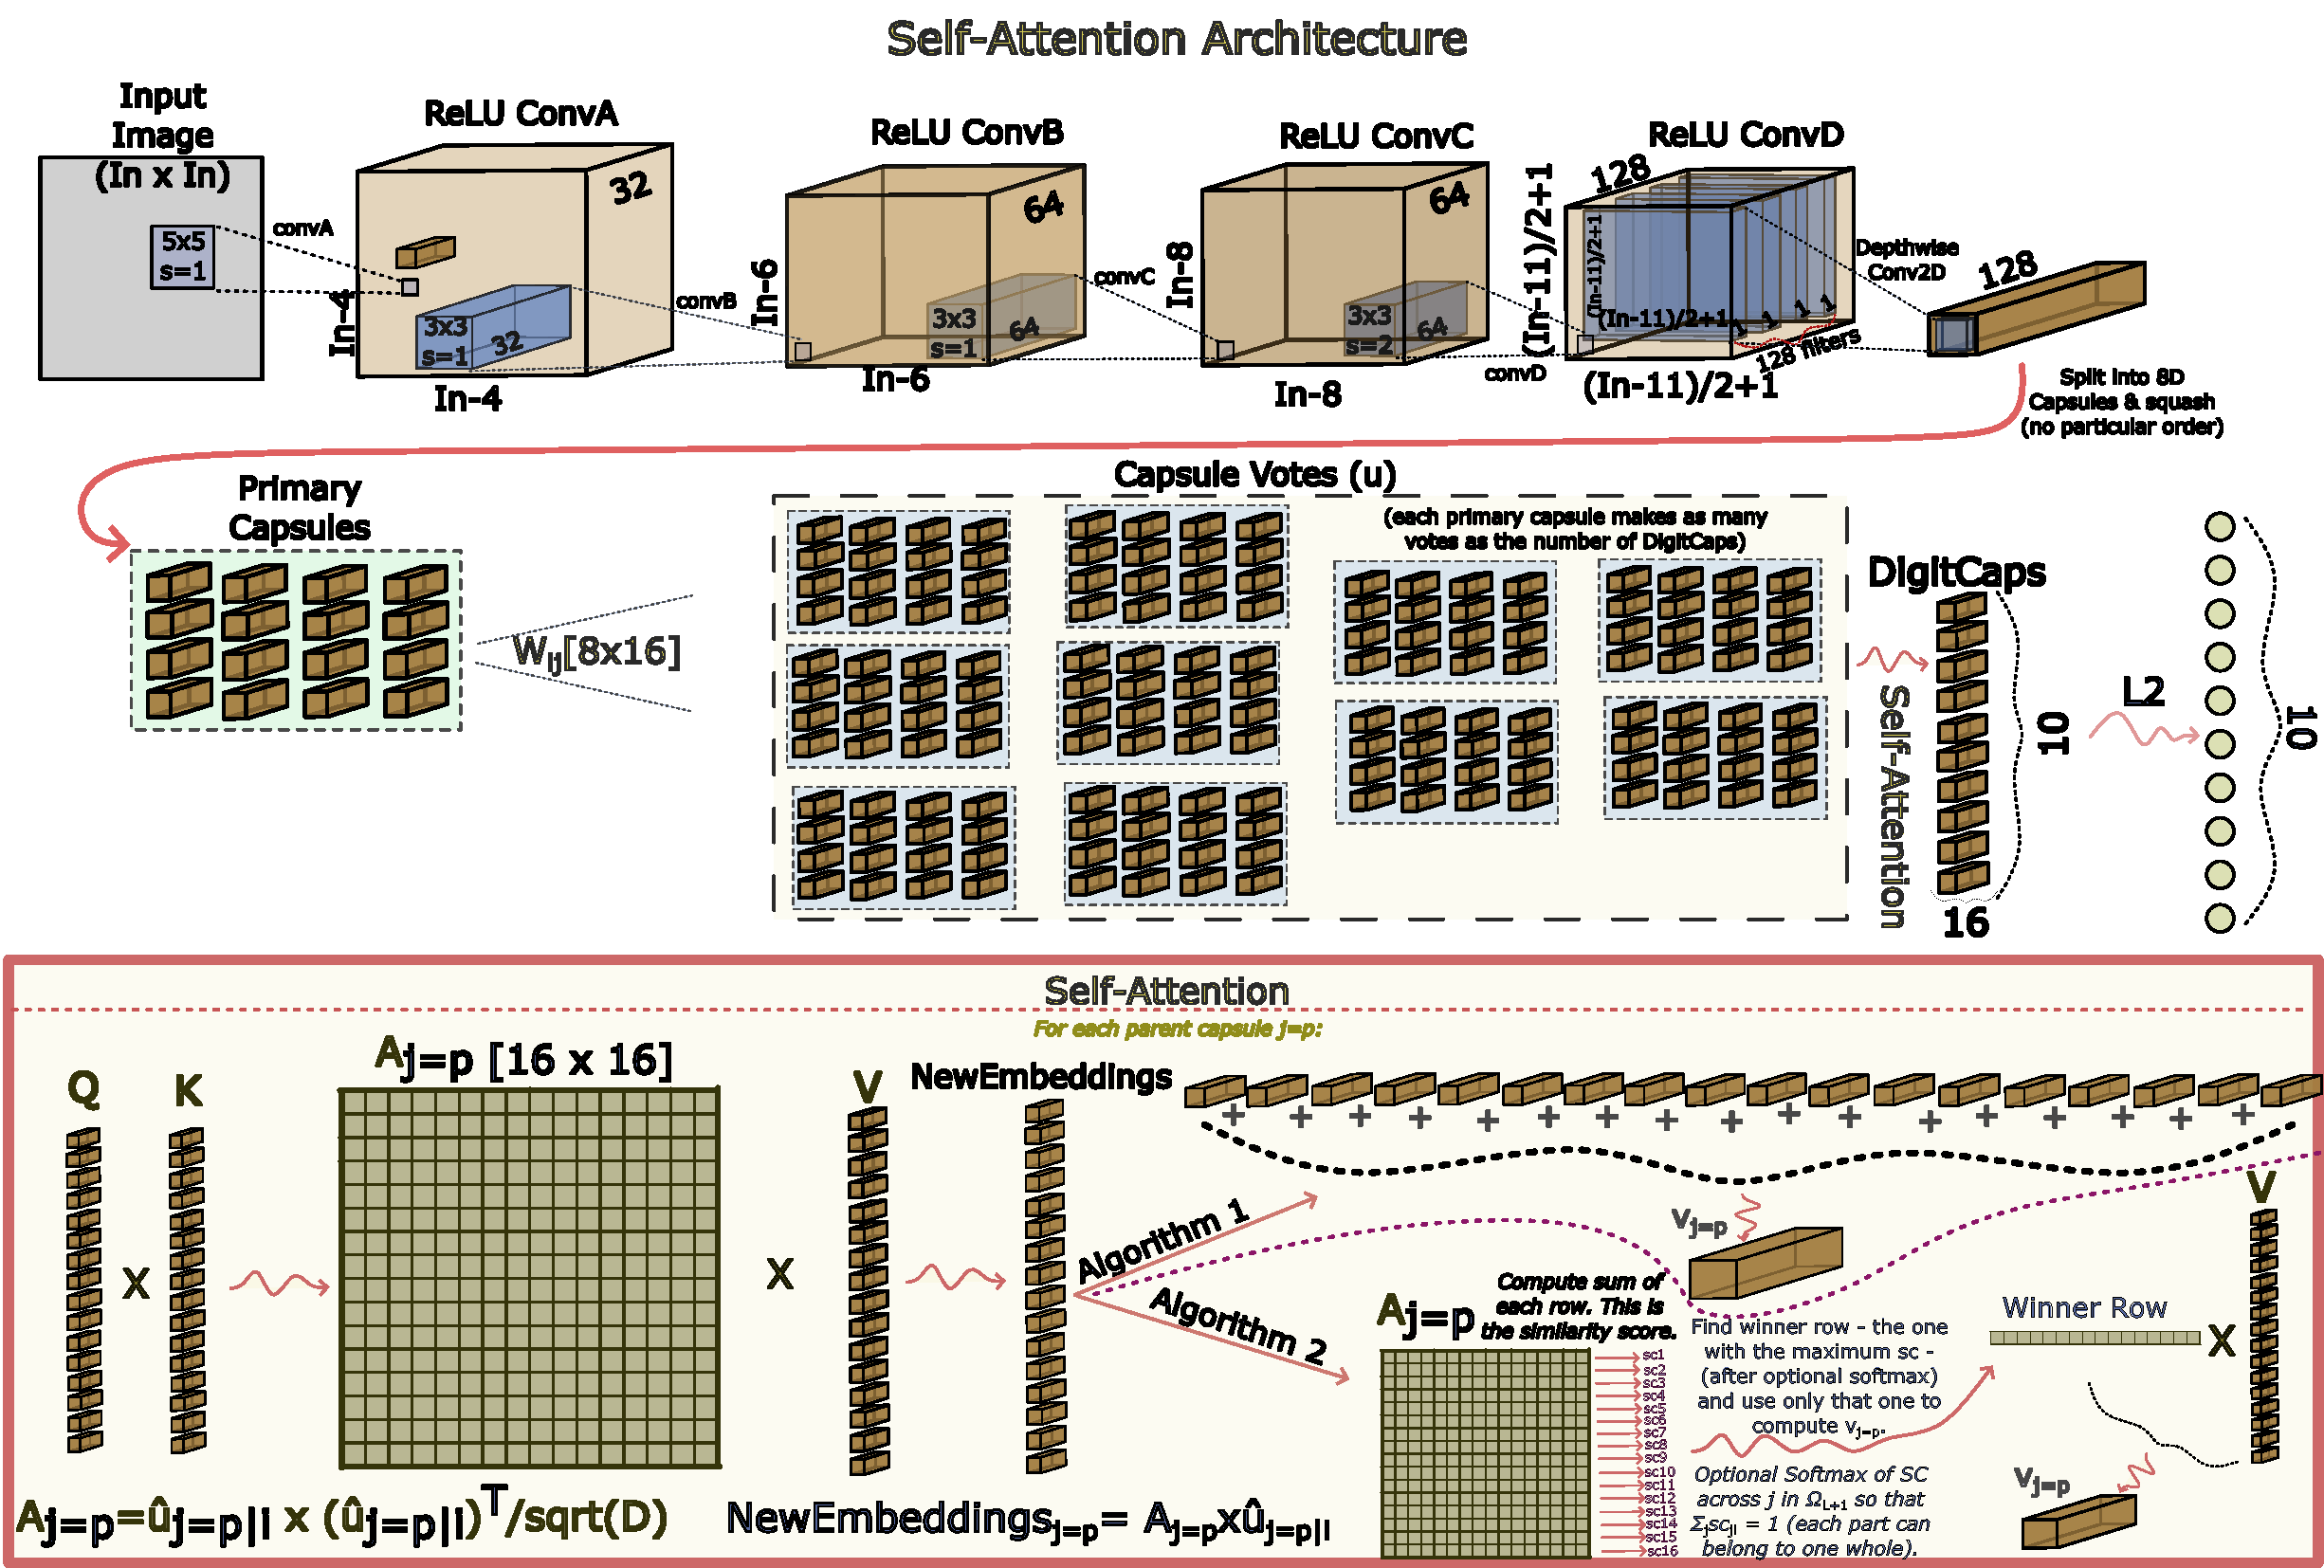
\includegraphics[width=0.97\textwidth]{images/chapter method/therd_method_architecture_encoder.pdf}
  \caption{Η αρχιτεκτονική του νευρωνικού δικτύου με κάψουλες της τρίτης μεθόδου. Στο σχήμα περιγράφονται σχηματικά οι δύο εναλλακτικοί αλγόριθμοι δρομολόγησης που αναπτύξαμε. Για λόγους απλότητας, δεν απεικονίζουμε την περίπτωση αυτο\textendash προσοχής πολλών κεφαλών. \textit{Παράχθηκε από το \href{https://inkscape.org/}{\en{Inkscape}}}.}
  \label{fig:method_3_architecture}
\end{figure}

Η βασική αρχιτεκτονική του δικτύου φαίνεται στο σχήμα \ref{fig:method_3_architecture}. Για τη μεταφορά από τον χώρο των εικονοστοιχείων στον χώρο των καψουλών χρησιμοποιούνται τέσσερα συνελικτικά επίπεδα και ένα επίπεδο συνέλιξης κατά βάθος (\en{Depthwise 2D convolution}). Οι συνήθεις παράμετροι των πρώτων συνελικτικών επιπέδων παρουσιάζονται στον πίνακα \ref{tab:method3_params}. Επισημαίνεται ότι μετά από κάθε συνελικτικό επίπεδο έχουμε ένα επίπεδο κανονικοποίησης κατά δέσμες (\en{batch normalization}). \par

\begin{table}[h]
  \begin{center}
    \begin{tabular}{| c | c c |} 
     \hline
     Επίπεδο & Πυρήνας & Αριθμός Φίλτρων \\ [0.5ex] 
     \hline\hline
     \en{A} & $5 \times 5$ & 32 \\ 
     \hline
     \en{B} & $3 \times 3$ & 64 \\
     \hline
     \en{C} & $3 \times 3$ & 64 \\
     \hline
     \en{D} & $3 \times 3$ & 128 \\ [1ex] 
     \hline
    \end{tabular}
    \caption{\label{tab:method3_params}Πίνακας στον οποίο παρουσιάζεται η παραμετροποίηση της αρχιτεκτονικής των πρώτων επιπέδων.}
    \end{center}
  \end{table}


Όπως προαναφέραμε, τα πρώτα τέσσερα επίπεδα διαδέχεται ένα επίπεδο συνέλιξης κατά βάθος. Ουσιαστικά, πρόκειται για ένα επίπεδο συνέλιξης με τόσα κυλιόμενα παράθυρα (δισδιάστατα φίλτρα) όση είναι και η διάσταση βάθους του προηγούμενου επιπέδου. Το καθένα από αυτά τα φίλτρα παράγει ένα χάρτη χαρακτηριστικών. Αξίζει να σημειωθεί ότι στην περίπτωσή μας, ακολουθώντας την υλοποίηση \cite{mazzia2021efficient}, το μέγεθος του κάθε δισδιάστατου πυρήνα το θέτουμε να είναι ίσο με τις διαστάσεις πλάτους και ύψους των χαρτών χαρακτηριστικών του προηγούμενου επιπέδου. Συνεπώς, από κάθε φίλτρο προκύπτει μια μονάδα (\en{scalar}). Συνολικά, δηλαδή, έχουμε σαν έξοδο έναν όγκο από αποκρίσεις (\en{activations}) μεγέθους $[1 \times 1 \times D_F]$, οπου $D_F$ ο αριθμός των φίλτρων του επιπέδου $D$. Το διάνυσμα αυτό το διαχωρίζουμε σε υποδιανύσματα με οκτώ στοιχεία το καθένα τα οποία και τροφοδοτούμε στη συνάρτηση σύνθλιψης (\en{squash}) σχηματίζοντας έτσι το πρώτο επίπεδο από κάψουλες (\en{PrimaryCapsules}).\par

Για παράδειγμα, στις περισσότερες παραμετροποιήσεις των πειραμάτων το συνελικτικό επίπεδο $D$ έχει σαν αποτέλεσμα τη δημιουργία 128 χαρτών χαρακτηριστικών μεγέθους $9 \times 9$. Τροφοδοτώντας αυτές τις αποκρίσεις σε ένα συνελικτικό επίπεδο κατά βάθος με 128 φίλτρα μεγέθους $9 \times 9$ λαμβάνουμε ένα διάνυσμα $128$ στοιχείων. Αυτό το διάνυσμα το χωρίζουμε σε κάψουλες διάστασης 8 με αποτέλεσμα να λάβουμε 16 \en{PrimaryCaps} (αφού πρώτα εφαρμόσουμε σε αυτές την τροποποιημένη συνάρτηση σύνθλιψης που εξηγούμε παρακάτω).\par

Η εν λόγω αρχιτεκτονική ενσωματώνει πολύ περισσότερα συνελικτικά επίπεδα από την αρχιτεκτονική που προτείνεται στο έργο \cite{sabour2017dynamic}. Παρόλα αυτά, μειώνοντας τον αριθμό των καψουλών που βρίσκονται στο πρώτο επίπεδο από κάψουλες, επιτυγχάνει να ελαττώσει σημαντικά τον αριθμό των εκπαιδευόμενων παραμέτρων. Για λόγους πειραματισμού, δοκιμάσαμε να μιμηθούμε τον τρόπο δημιουργίας του επιπέδου \en{PrimaryCaps} που χρησιμοποιείται στο έργο \cite{sabour2017dynamic}, όπως τον περιγράψαμε στην πρώτη μέθοδο του παρόντος κεφαλαίου. Έτσι, στη θέση των τεσσάρων συνελικτικών επιπέδων έχουμε ένα επίπεδο από 256 φίλτρα με πυρήνες $9 \times 9$ (βλέπε σχήμα \ref{fig:method_1_architecture}). Θα αναφερόμαστε σε αυτήν την αρχιτεκτονική ως \textquote{εναλλακτική αρχιτεκτονική} σε αντιπαραβολή με τη \textquote{βασική αρχιτεκτονική} που απεικονίζεται στο σχήμα \ref{fig:method_3_architecture}.\par

Συνεχίζοντας την περιγραφή της αρχιτεκτονικής από τα αριστερά προς τα δεξιά, μέσω του αλγορίθμου δρομολόγησης με μηχανισμό αυτο\textendash προσοχής διαμορφώνονται οι κάψουλες του τελευταίου επιπέδου (ονομάζονται και \en{DigitCaps}). Αναπόσπαστο στοιχείο της διαδικασίας σχηματισμού των καψουλών του ανώτερου επιπέδου είναι ο υπολογισμός των ψήφων για την πόζα των \en{DigitCaps}. Κατά αναλογία με την υλοποίηση \cite{sabour2017dynamic}, η κάθε κάψουλα επιπέδου \en{PrimaryCaps} χρησιμοποιώντας πίνακες μετασχηματισμού με εκπαιδευόμενα βάρη παράγει μια πρόβλεψη για κάθε κάψουλα επιπέδου \en{DigitCaps}. Αυτές οι ψήφοι στη συνέχεια φιλτράρονται μέσω ενός γρήγορου αλγορίθμου δρομολόγησης με αυτο\textendash προσοχή (αναλύεται παρακάτω) και σχηματίζονται οι κάψουλες του τελικού επιπέδου.

\subsection{Αλγόριθμοι Δρομολόγησης}

Μια σημαντική αδυναμία των νευρωνικών δικτύων με κάψουλες που διαπιστώθηκε κατά τη μελέτη σχετικής βιβλιογραφίας είναι αυτή της κλιμάκωσης σε μεγαλύτερες διατάξεις. Τροχοπέδη για την κλιμάκωση αποτελεί το αυξημένο υπολογιστικό κόστος και η αστάθεια των επαναληπτικών αλγορίθμων δρομολόγησης. Επιδιώκοντας να δοθεί λύση στο πρόβλημα, παρατηρήσαμε την πρόσφατη άνθιση των μοντέλων νευρωνικών δικτύων που χρησιμοποιούν μηχανισμό αυτο\textendash προσοχής (υπό τη μορφή μετασχηματιστών) τόσο για εφαρμογές επεξεργασίας φυσικής γλώσσας (\en{natural language processing}) όσο και για εφαρμογές όρασης υπολογιστών (\en{computer vision}). Συγκεκριμένα,  σημαντική πηγή έμπνευσης αποτέλεσαν τα έργα \cite{dosovitskiy2020image_is_worth_16, carion2020end}. Δανειζόμενοι στοιχεία από τη χρήση μηχανισμού αυτο\textendash προσοχής σε εικόνες και διατηρώντας παράλληλα τις βασικές υποθέσεις των νευρωνικών δικτύων με κάψουλες επινοήσαμε μια οικογένεια από γρήγορους, κλιμακώσιμους (\en{scalable}) και μη\textendash επαναληπτικούς αλγορίθμους δρομολόγησης.\par

Όπως γίνεται αντιληπτό από το κεφάλαιο \ref{chap:related_work}, δεν είναι η πρώτη φορά που χρησιμοποιείται μηχανισμός αυτο\textendash προσοχής στο πλαίσιο των νευρωνικών δικτύων με κάψουλες. Στα έργα \cite{hoogi2019self, huang2020capsnet} χρησιμοποιείται ο εν λόγω μηχανισμός ως επίπεδο που προηγείται του σχηματισμού των \en{PrimaryCaps}, το οποίο διαφέρει σημαντικά από την υλοποίησή μας που ενσωματώνει τον μηχανισμό αυτο\textendash προσοχής στον αλγόριθμο δρομολόγησης. Επίσης, αν και η υλοποίησή μας άντλησε στοιχεία από το έργο \cite{mazzia2021efficient} (το μόνο που εφαρμόζει τον μηχανισμό στον αλγόριθμο δρομολόγησης) είναι πολύ πιο πιστή στις βασικές υποθέσεις των δικτύων με κάψουλες. Εν αντιθέσει, για τον αλγόριθμο δρομολόγησης των \en{Mazzia et al.} (τον ονομάζουμε \textquote{απλοϊκό αλγόριθμο δρομολόγησης με αυτο\textendash προσοχή}) δεν καταφέραμε να δώσουμε μια λογική εξήγηση ου να συμφωνεί με τις αρχές των νευρωνικών δικτύων με κάψουλες. Επίσης, όπως θα φανεί στο επόμενο κεφάλαιο, η υλοποίησή μας με παρόμοιο αριθμό παραμέτρων επιτυγχάνει καλύτερες επιδόσεις (χωρίς ιδιαίτερο πειραματισμό των παραμέτρων).\par

Στην παρούσα υποενότητα θα παρουσιάσουμε τους δύο εναλλακτικούς αλγορίθμους που αναπτύξαμε καθώς και τη λογική πίσω από τον καθένα. Επίσης, για λόγους πληρότητας, θα παρουσιάσουμε τον \textquote{απλοϊκό αλγόριθμο δρομολόγησης με αυτο\textendash προσοχή} που χρησιμοποιείται στην υλοποίηση \cite{mazzia2021efficient}. Προτού όμως ξεκινήσουμε την παρουσίαση, κρίνεται σκόπιμο να ορίσουμε τον συμβολισμό που θα χρησιμοποιηθεί σε όλη την έκταση των αλγορίθμων μας. Χρησιμοποιούμε τον δικό μας συμβολισμό ο οποίος διαφέρει από αυτών των προηγούμενων αλγορίθμων καθώς δεν ήταν επαρκής ώστε να περιγράψει τις νέες έννοιες που εισάγουμε. Έτσι έχουμε:
\begin{itemize}
  \item Σαν σύμβαση, χρησιμοποιούμε τον δείκτη $i$ για να αναφερθούμε σε κάψουλες επιπέδου $L$ και τον δείκτη $j$ για τις κάψουλες επιπέδου $L+1$.
  \item Το σύνολο των καψουλών ενός επιπέδου $L$ το συμβολίζουμε ως $\Omega_L$ και τον πληθάριθμο του συνόλου (\en{cardinality}) ως $n^L = \left\lvert \Omega_L \right\rvert$.
  \item Τις επιμέρους κάψουλες ενός επιπέδου $L$ τις συμβολίζουμε με $C^L_i$ ενώ με $C^L$ συμβολίζουμε τη μήτρα στην οποία οργανώνονται όλες οι κάψουλες επιπέδου $L$. Το μέγεθος της κάθε κάψουλας επιπέδου $L$ (μήκος του διανύσματος με το οποίο αναπαρίσταται η κάψουλα) συμβολίζεται με $d^L$.
  \item Μεταξύ δύο επιπέδων από κάψουλες $L$ και $L+1$, κάθε κάψουλα $C^L_i \in \Omega_L$ προβλέπει ποια θα είναι η πόζα της κάθε κάψουλας $C^{L+1}_j \in \Omega_{L+1}$. Έτσι προκύπτουν $n^L \times n^{L+1}$ προβλέψεις (ή ψήφοι) όπου την κάθε μια τη συμβολίζουμε με $V_{ij}^L$. Αυτές οι ψήφοι οργανώνονται στη μήτρα $V^L$ η οποία όπως είναι λογικό, περιέχει $n^L \times n^{L+1}$ κάψουλες - ψήφους: $n^L$ ψήφους για κάθε κάψουλα $C^{L+1}_i$.
  \item Σε περίπτωση που θα θέλαμε να αναφερθούμε σε όλες τις ψήφους που αφορούν μια κάψουλα επιπέδου $L+1$ αρκεί να \textquote{δεσμεύσουμε} την ελεύθερη μεταβλητή $j$ και να γράψουμε $V^L_j$ (ή, καλύτερα, $V^L_{:j}$ ώστε να είναι εμφανές ότι η μεταβλητή $i$ που αφορά τις κάψουλες επιπέδου $L$ παραμένει ελεύθερη). Κατά αντιστοιχία, αν θα θέλαμε να αναφερθούμε στις ψήφους που προκύπτουν από την κάψουλα $C^L_i$ θα γράφαμε $V^L_i$ (ή, σαφέστερα, $V^L_{i:}$). Κατά αυτόν τον τρόπο, αν δεσμεύσουμε όλες τις διαστάσεις μιας μήτρας, τότε έχουμε ένα βαθμωτό μέγεθος. Για παράδειγμα, έστω κάψουλες $C^L \in \Re^{n^L \times d^L}$. Τότε αν δεσμεύσουμε την ελεύθερη μεταβλητή $i \in [1, n^L]$ τότε ισχύει $C_i^L \in \Re^{d^L}$. Αν δεσμεύσουμε και το επιμέρους τμήμα του διανύσματος της κάψουλας λαμβάνουμε έναν πραγματικό αριθμό, δηλαδή: $C_{ik}^L \in \Re$ \footnote{Μάλιστα είναι $C_{ik}^L \in [0,1]$ αφού η συνάρτηση \en{squash} δεν επιτρέπει τα διανύσματα των καψουλών να έχουν μήκος μεγαλύτερο της μονάδας.}.
  \item Όπως γίνεται κατανοητό από το ανωτέρω παράδειγμα, ο δείκτης $k_L$ θα χρησιμοποιείται για να αναφερόμαστε στα επιμέρους στοιχεία ενός διανύσματος μεγέθους $d^L$.
  \item Οι πίνακες από βάρη ενός επιπέδου $L$ που αποθηκεύουν τις σχέσεις μέρους - όλου οργανώνονται στη μήτρα $W^L$. Η μήτρα περιέχει όλα τα επιμέρους βάρη $W_{ij}^L$ που χρησιμοποιούν οι κάψουλες $C^L$ για να παράξουν τις προβλέψεις $V^L$. Για μια κάψουλα $c_i^L \in \Omega_L$, η ψήφος της υπολογίζεται με τη φόρμουλα: $V_{ij}^L = C_i^L \times W_{ij}^L$.
  \item Συνήθως, μπορεί να αναφερόμαστε στις κάψουλες επιπέδου $L$ ως κάψουλες παιδιά και στις αντίστοιχες του επιπέδου $L+1$ ως κάψουλες γονείς.
  \item Ο επιμέρους πίνακας που προκύπτει από τον μηχανισμό αυτο\textendash προσοχής των ψήφων $V^L_j$ για μια κάψουλα $C_j^{L+1}$ συμβολίζεται ως $Α^L_j$. Η μήτρα που περιέχει όλους τους πίνακες προσοχής ($\forall C_j^{L+1} \in \Omega_{L+1}$) συμβολίζεται με $A^L$.
  \item Στην περίπτωση που χρησιμοποιείται αυτο\textendash προσοχή πολλών κεφαλών (\en{multi\textendash head self\textendash attention}) η αναφορά σε επιμέρους κεφαλές γίνεται με τον δείκτη $h$. Για παράδειγμα, η πρώτη κεφαλή (\en{head}) ενός πίνακα προσοχής για μια κάψουλα $C^{L+1}_j$ συμβολίζεται ως $A_{jh=1}^L$.
  \item Η μήτρα βαρών δρομολόγησης μεταξύ επιπέδων $L$ και $L + 1$ συμβολίζεται με $\mathbf{R}^L$. Αυτή, μεταξύ δύο πλήρως διασυνδεδεμένων επιπέδων από κάψουλες, περιέχει όλα τα βάρη ακμών τα οποία συμβολίζονται με $\mathbf{R}_{ij}^L$.
\end{itemize}


\subsubsection{Απλοϊκός αλγόριθμος δρομολόγησης με αυτο\textendash προσοχή}

Στην παράγραφο αυτή γίνεται αναφορά στον αλγόριθμο που χρησιμοποιεί το έργο \cite{mazzia2021efficient}. Σε γενικές γραμμές, πρόκειται για τον μη\textendash επαναληπτικό αλγόριθμο ο οποίος χρησιμοποιεί τον μηχανισμό αυτο\textendash προσοχής προκειμένου να υπολογίσει τα βάρη δρομολόγησης (\en{coupling coefficients}). Αν και το έργο δεν προσφέρει μια πειστική, λογική εξήγηση για όλα τα βήματα του αλγορίθμου, οι υψηλές επιδόσεις του παρακίνησαν την κατασκευή των εξελιγμένων αλγορίθμων που παρουσιάζουμε σε επόμενες παραγράφους.\par

\en{
\begin{algorithm}[hp]
  \caption{\gr{Απλοϊκός Αλγόριθμος Δρομολόγησης με Αυτο\textendash προσοχή}}\label{alg:method3_stupid_routing}
  \hspace*{\algorithmicindent} \textbf{Input} PrimaryCaps $C^L \in \Re^{n^L \times d^L}$\\
  \hspace*{\algorithmicindent} \textbf{Output} DigitCaps $C^{L+1} \in \Re^{n^{L+1} \times d^{L+1}}$\\
  \hspace*{\algorithmicindent} \textbf{Trainable Parameters} $W^L \in \Re^{n^{L+1} \times n^L \times d^L \times d^{L+1}}, b^L \in \Re^{n^{L+1} \times n^L}$

  \begin{algorithmic}[1]
    % \item[] % Empty, unnumbered line
    \Procedure{Main}{$C^L$} \Comment{Input: $C^L \in  \Re^{n^L \times d^L}$} 
      \State $V^L \gets$ \Call{ComputeVotes}{$C^L$}
      \State $A^L \gets$ \Call{Self-Attention}{$V^L$}
      \State $\textbf{R}^L \gets$ \Call{ComputeRootingCoefficients}{$A^L$}
      \State $\forall j \in \Omega_{L+1}: S_j^{L+1} \gets (\textbf{R}_j^L + b_j^L) \times V_j^L$ \Comment{Equiv.: $S_{jk}^{L+1} \gets \sum_i^{n^L} (\textbf{R}_{ji}^L + b_{ji}^L) \ast V_{jik}^L$}
      \State $\forall j \in \Omega_{L+1}: C_j^{L+1} \gets squash(S_j^{L+1})$
      \State \Return $C^{L+1}$ \Comment{Output: $C^{L+1} \in  \Re^{n^{L+1} \times d^{L+1}}$} 
    \EndProcedure
    % \item[] % Empty, unnumbered line
    \Procedure{ComputeVotes}{$C^L$}  \Comment{Input: $C^L \in  \Re^{n^L \times d^L}$} 
      \State $\forall j \in \Omega_{L+1}, \forall i \in \Omega_L: V_{ji:}^L \gets C_{i:}^L \times W_{ji::}^L$ \Comment{Equiv.: $V^L_{jik_{L+1}} \gets \sum_{k_{L}}^{d^L} C_{ik_L}^L \ast W_{jik_Lk_{L+1}}$}
      \State \Return $V^{L}$ \Comment{Output: $V^{L} \in \Re^{n^{L+1} \times n^{L} \times d^{L+1}}$}
    \EndProcedure
    
    \Procedure{Self-Attention}{$V^L$}  \Comment{Input: $V^L \in \Re^{n^{L+1} \times n^L \times d^{L+1}}$} 
      \State $\forall j \in \Omega_{L+1}: A_j^L \gets \frac{V^L_j \times {V_j^{L}}^T}{\sqrt{d^{L+1}}}$ \Comment{Equiv.: $A^L_{ji_1i_2} \gets \sum_k^{d^{L+1}} V^L_{ji_1k} \ast V^L_{ji_2k}$}
      \State \Return $A^{L}$ \Comment{Output: $A^{L} \in \Re^{n^{L+1} \times n^{L} \times n^{L}}$}
    \EndProcedure

    \Procedure{ComputeRootingCoefficients}{$A^L$} \Comment{Input: $A^{L} \in \Re^{n^{L+1} \times n^{L} \times n^{L}}$}
      \State $\forall j \in \Omega_{L+1}: R_j^L \gets \sum_{i_1}^{n^L} A^L_{ji_1:}$ \Comment{Equiv.: $R_{ji_2}^L \gets \sum_{i_1}^{n^L} A^L_{ji_1i_2}$} \label{op:stupid_algo_is_sum_of_rows}
      \State $\forall i \in \Omega_{L}: \mathbf{R}_{:i}^L \gets \mathit{softmax}(R_{:i}^L)$ \Comment{Equiv.: $\mathbf{R}_{ji}^L \gets \frac{\exp(R_{ji}^L)}{\sum_j^{n^{L+1}} \exp(R_{ji}^L)}$} \label{op:stupid_algo_softmax_definition}% How to define softmax: $\mathit{softmax}(X \in \Re^{1\times n}) = $
      \State \Return $\mathbf{R}^L$ \Comment{Output: $\mathbf{R}^{L} \in \Re^{n^{L+1} \times n^{L}}$}
    \EndProcedure

  \end{algorithmic}
  \end{algorithm}
}


Αν και τα ανωτέρω βήματα έχουν παρουσιαστεί πολύ αναλυτικά με ισοδύναμες (\en{"Equivalent"}), σημειακές εκφράσεις, μπορούμε να κάνουμε τα παρακάτω σχόλια:
\begin{itemize}
  \item Το σύμβολο $\ast$ συμβολίζει τον πολλαπλασιασμό μεταξύ δύο βαθμωτών μεγεθών (\en{scalars}).
  \item Η συνάρτηση $softmax()$ στο βήμα \ref{op:stupid_algo_softmax_definition} σκοπό έχει να επιβάλει τον περιορισμό $\sum_j^{n^{L+1}} R_{ji} = 1$ και να ενισχύσει το βάρος δρομολόγησης με το μεγαλύτερο μέτρο έτσι ώστε, τελικά, μια κάψουλα παιδί να μην ανήκει ολοκληρωτικά σε πολλούς γονείς (\en{single parent assumption}). Σε τεχνικό επίπεδο, η συνάρτηση δέχεται σαν είσοδο ένα διάνυσμα στήλη και μπορεί να οριστεί ως εξής:
  \begin{equation}
    \mathit{softmax}(X \in \Re^{n \times 1}) = \frac{\exp(X_k)}{\sum_k^n \exp(X_k)}.
  \end{equation}
  \item Στη γραμμή \ref{op:stupid_algo_is_sum_of_rows} του αλγορίθμου, το αριστερό άθροισμα διενεργείται σημειακά σε διανύσματα γραμμές. Ουσιαστικά, για μια κάψουλα γονέα $j$, οι ομοιότητες της εκάστοτε ψήφου από την κάψουλα $C_i^L$ με τις άλλες ψήφους από τις κάψουλες $C_{\acute{i}}^L \in \Omega_L \setminus C_i^L$ αθροίζονται στην τιμή $R_{ji}^L$. Η ποιοτική ερμηνεία αυτής της πράξης δεν αναλύεται στο έργο \cite{mazzia2021efficient}. Σε μια προσπάθεια ερμηνείας, θα μπορούσαμε να αναφέρουμε ότι κάθε θέση $i$ του διανύσματος γραμμής $R_j^L$ που προκύπτει, φανερώνει ποιες ψήφοι καψουλών $C_i^L$ εμφανίζουν μεγάλη ομοιότητα με τις υπόλοιπες ψήφους για το συγκεκριμένο το $j$. Έτσι, στη συνέχεια, η κάθε κάψουλα $C_j^{L+1}$ θα συντίθεται μόνο από τις ψήφους των $C_{i}^L$ που εμφάνιζαν μεγάλη ομοιότητα με τις υπόλοιπες ψήφους από τις κάψουλες $C_{\acute{i}}^L \in \Omega_L \setminus C_i^L$ (πάντα για συγκεκριμένο $j$).
\end{itemize}

Πλέον, είμαστε σε θέση να παρουσιάσουμε τους δικούς μας αλγορίθμους οι οποίοι έχουν περισσότερο προφανή ποιοτική ερμηνεία και μάλιστα, επιτυγχάνουν καλύτερα πειραματικά αποτελέσματα.

\subsubsection{Αλγόριθμος Δρομολόγησης με Αυτο\textendash προσοχή 1 (Αλγόριθμος \en{RooMAV})}

\en{
\begin{algorithm}[hp]
  \caption{\gr{Αλγόριθμος Δρομολόγησης με Αυτο\textendash προσοχή 1 (Αλγόριθμος \en{RooMAV}) }}\label{alg:method3_sum_routing}
  \hspace*{\algorithmicindent} \textbf{Input} PrimaryCaps $C^L \in \Re^{n^L \times d^L}$\\
  \hspace*{\algorithmicindent} \textbf{Output} DigitCaps $C^{L+1} \in \Re^{n^{L+1} \times d^{L+1}}$\\
  \hspace*{\algorithmicindent} \textbf{Trainable Parameters} $W^L \in \Re^{n^{L+1} \times n^L \times d^L \times d^{L+1}}$
  \begin{algorithmic}[1]
    % \item[] % Empty, unnumbered line
    \Procedure{Main-RooMAV}{$C^L$} \Comment{Input: $C^L \in  \Re^{n^L \times d^L}$} 
      \State $V^L \gets$ \Call{ComputeVotes}{$C^L$}
      \State $A^L \gets$ \Call{Self-Attention}{$V^L$}
      \State $\prescript{+}{}{A^{L}} \gets$ \Call{ComputeNonNegativeAttentionMap}{$A^L$}
      \State $E^L \gets$ \Call{NewEmb}{$\prescript{+}{}{A^{L}}, V^L$} \Comment{Computes new, context-aware, votes.}
      \State $\forall j \in \Omega_{L+1}: S^{L+1}_j \gets \sum_i^{n^L} E^L_{ji}$ \Comment{Equiv.: $S^{L+1}_{jk} \gets \sum_i^{n^L} E^L_{jik}$}
      \State $\forall j \in \Omega_{L+1}: C_j^{L+1} \gets squash(S_j^{L+1})$
      \State \Return $C^{L+1}$ \Comment{Output: $C^{L+1} \in  \Re^{n^{L+1} \times d^{L+1}}$} 
    \EndProcedure
    % \item[] % Empty, unnumbered line
    \Procedure{ComputeVotes}{$C^L$}  \Comment{Input: $C^L \in  \Re^{n^L \times d^L}$} 
      \State $\forall j \in \Omega_{L+1}, \forall i \in \Omega_L: V_{ji:}^L \gets C_{i:}^L \times W_{ji::}^L$ \Comment{Equiv.: $V^L_{jik_{L+1}} \gets \sum_{k_{L}}^{d^L} C_{ik_L}^L \ast W_{jik_Lk_{L+1}}$}
      \State \Return $V^{L}$ \Comment{Output: $V^{L} \in \Re^{n^{L+1} \times n^{L} \times d^{L+1}}$}
    \EndProcedure
    
    \Procedure{Self-Attention}{$V^L$}  \Comment{Input: $V^L \in \Re^{n^{L+1} \times n^L \times d^{L+1}}$} 
      \State $\forall j \in \Omega_{L+1}: A_j^L \gets \frac{V^L_j \times {V_j^L}^T}{\sqrt{d^{L+1}}}$ \Comment{Equiv.: $A^L_{ji_1i_2} \gets \sum_k^{d^{L+1}} V^L_{ji_1k} \ast V^L_{ji_2k}$}
      \State \Return $A^{L}$ \Comment{Output: $A^{L} \in \Re^{n^{L+1} \times n^{L} \times n^{L}}$}
    \EndProcedure

    \Procedure{ComputeNonNegativeAttentionMap}{$A^L$}\Comment{Input: $A^{L} \in \Re^{n^{L+1} \times n^{L} \times n^{L}}$}
      \State $\forall j \in \Omega_{L+1}:  \prescript{+}{}{A^{L}_j} \gets \mathbf{ReLU}(A^L_j)$ \Comment{Equiv.: $\prescript{+}{}{A^{L}_{ji\tilde{i}}} \gets ReLU(A^L_{ji\tilde{i}})$} \label{op:method3_sum_pointwise_relu_this_op_may_be_different}
      \State \Return $\prescript{+}{}{A^{L}}$ \Comment{Output: $\prescript{+}{}{A^{L}} \in \Re^{n^{L+1} \times n^{L} \times n^{L}}$}
    \EndProcedure

    \Procedure{NewEmb}{$\prescript{+}{}{A^{L}}, V^L$} \Comment{Input: $\prescript{+}{}{A^{L}} \in \Re^{n^{L+1} \times n^{L} \times n^{L}}, V^L \in \Re^{n^{L+1} \times n^L \times d^{L+1}}$} 
    \State $\forall j \in \Omega_{L+1}: E^L_j \gets \prescript{+}{}{A_j^L} \times V_j^L$ \Comment{Equiv.: $E^L_{jik} \gets \sum_{\tilde{i}}^{n^L} \prescript{+}{}{A_{ji\tilde{i}}^L} \ast V^L_{j\tilde{i}k}$} \label{op:method3_sum_weighted_sum} % Πες για την ερμηνεία, πρόκειται για σταθμισμένο άθροισμα των votes. Αλλά εσύ το κάνες για κάθε ένα row. Υπολογίζεις μια νέα αναπαράσταση (embeding) που είναι context-aware, δηλαδή σχηματίζεται από όλες τις ψήφους (για την κάψουλα j) που συμφωνούν με την εκάστοτε κάψουλα i (εκπρόσωπος γραμμής). Από εδώ είναι εύκολο να πας λογικά στον επόμενο αλγόριθμο που βρίσκει το max row.
    \State \Return $E^L$ \Comment{Output: $E^{L} \in \Re^{n^{L+1} \times n^{L} \times d^{L+1}}$}
    \EndProcedure

  \end{algorithmic}
  \end{algorithm}
}

\subsubsection{Αλγόριθμος Δρομολόγησης με Αυτο\textendash προσοχή 2 (Αλγόριθμος \en{RoWSS})}

\en{
\begin{algorithm}[hp]
  \caption{\gr{Αλγόριθμος Δρομολόγησης με Αυτο\textendash προσοχή 2 (Αλγόριθμος \en{RoWSS})}}\label{alg:method3_max_rooting}
  \hspace*{\algorithmicindent} \textbf{Input} PrimaryCaps $C^L \in \Re^{n^L \times d^L}$\\
  \hspace*{\algorithmicindent} \textbf{Output} DigitCaps $C^{L+1} \in \Re^{n^{L+1} \times d^{L+1}}$\\
  \hspace*{\algorithmicindent} \textbf{Trainable Parameters} $W^L \in \Re^{n^{L+1} \times n^L \times d^L \times d^{L+1}}$
  \begin{algorithmic}[1]
    % \item[] % Empty, unnumbered line
    \Procedure{Main-RoWSS}{$C^L$} \Comment{Input: $C^L \in  \Re^{n^L \times d^L}$} 
      \State $V^L \gets$ \Call{ComputeVotes}{$C^L$}
      \State $A^L \gets$ \Call{Self-Attention}{$V^L$}
      \State $\prescript{+}{}{A^{L}} \gets$ \Call{ComputeNonNegativeAttentionMap}{$A^L$}
      \State $E^L \gets$ \Call{NewEmb}{$\prescript{+}{}{A^{L}}, V^L$} \Comment{Computes new, context-aware, votes.}
      \State $Winners^L \gets$ \Call{FindWinnerIndexes}{$\prescript{+}{}{A^{L}}$}
      \State $\forall j \in \Omega_{L+1}: S^{L+1}_j \gets E^L_{ji=Winners_j^L}$ \Comment{Equiv.: $S^{L+1}_{jk} \gets E^L_{ji=Winners_j^Lk}$}
      \State $\forall j \in \Omega_{L+1}: C_j^{L+1} \gets squash(S_j^{L+1})$
      \State \Return $C^{L+1}$ \Comment{Output: $C^{L+1} \in  \Re^{n^{L+1} \times d^{L+1}}$} 
    \EndProcedure
    % \item[] % Empty, unnumbered line
    \Procedure{ComputeVotes}{$C^L$}  \Comment{Input: $C^L \in  \Re^{n^L \times d^L}$} 
      \State $\forall j \in \Omega_{L+1}, \forall i \in \Omega_L: V_{ji:}^L \gets C_{i:}^L \times W_{ji::}^L$ \Comment{Equiv.: $V^L_{jik_{L+1}} \gets \sum_{k_{L}}^{d^L} C_{ik_L}^L \ast W_{jik_Lk_{L+1}}$}
      \State \Return $V^{L}$ \Comment{Output: $V^{L} \in \Re^{n^{L+1} \times n^{L} \times d^{L+1}}$}
    \EndProcedure
    
    \Procedure{Self-Attention}{$V^L$}  \Comment{Input: $V^L \in \Re^{n^{L+1} \times n^L \times d^{L+1}}$} 
      \State $\forall j \in \Omega_{L+1}: A_j^L \gets \frac{V^L_j \times {V_j^L}^T}{\sqrt{d^{L+1}}}$ \Comment{Equiv.: $A^L_{ji_1i_2} \gets \sum_k^{d^{L+1}} V^L_{ji_1k} \ast V^L_{ji_2k}$}
      \State \Return $A^{L}$ \Comment{Output: $A^{L} \in \Re^{n^{L+1} \times n^{L} \times n^{L}}$}
    \EndProcedure

    \Procedure{ComputeNonNegativeAttentionMap}{$A^L$}\Comment{Input: $A^{L} \in \Re^{n^{L+1} \times n^{L} \times n^{L}}$}
    \State $\forall j \in \Omega_{L+1}:  \prescript{+}{}{A^{L}_j} \gets \mathbf{ReLU}(A^L_j)$ \Comment{Equiv.: $\prescript{+}{}{A^{L}_{ji\tilde{i}}} \gets ReLU(A^L_{ji\tilde{i}})$} \label{op:method3_max_pointwise_relu_this_op_may_be_different}
    \State \Return $\prescript{+}{}{A^{L}}$ \Comment{Output: $\prescript{+}{}{A^{L}} \in \Re^{n^{L+1} \times n^{L} \times n^{L}}$}
    \EndProcedure

    \Procedure{NewEmb}{$\prescript{+}{}{A^{L}}, V^L$} \Comment{Input: $\prescript{+}{}{A^{L}} \in \Re^{n^{L+1} \times n^{L} \times n^{L}}, V^L \in \Re^{n^{L+1} \times n^L \times d^{L+1}}$} 
    \State $\forall j \in \Omega_{L+1}: E^L_j \gets \prescript{+}{}{A_j^L} \times V_j^L$ \Comment{Equiv.: $E^L_{jik} \gets \sum_{\tilde{i}}^{n^L} \prescript{+}{}{A_{ji\tilde{i}}^L} \ast V^L_{j\tilde{i}k}$} \label{op:method3_max_weighted_sum} % Πες για την ερμηνεία, πρόκειται για σταθμισμένο άθροισμα των votes. Αλλά εσύ το κάνες για κάθε ένα row. Υπολογίζεις μια νέα αναπαράσταση (embeding) που είναι context-aware, δηλαδή σχηματίζεται από όλες τις ψήφους (για την κάψουλα j) που συμφωνούν με την εκάστοτε κάψουλα i (εκπρόσωπος γραμμής). Από εδώ είναι εύκολο να πας λογικά στον επόμενο αλγόριθμο που βρίσκει το max row.
    \State \Return $E^L$ \Comment{Output: $E^{L} \in \Re^{n^{L+1} \times n^{L} \times d^{L+1}}$}
    \EndProcedure

    \Procedure{FindWinnerIndexes}{$A^L$} \Comment{Input: $A^{L} \in \Re^{n^{L+1} \times n^{L} \times n^{L}}$}
    \State $\forall j \in \Omega_{L+1}: SC_j^L \gets (\sum_{i_2}^{n^L} A^L_{j:i_2})^T$ \Comment{Equiv.: $SC_{ji}^L \gets \sum_{i_2}^{n^L} A^L_{jii_2}$} \label{op:method3_max_sum_of_vector_columns} % Επίσης, πες που ανήκει το SC (διαστάσεις). Πες ότι το άθροισμα αριστερά είναι ισοδύναμο με το  $\forall j \in \Omega_{L+1}: SC_j^L \gets \sum_{i_1}^{n^L} A^L_{ji_1:}$ επειδή ο πίνακας Α είναι συμμετρικός (άθροισμα γραμμών == άθροισμα στηλών).
    \State \Comment{$SC^L \in \Re^{n^{L+1} \times n^L}$}
    \State $\forall i \in \Omega_L: SoftSC_{:i}^L \gets softmax(SC^L_{:i})$ \Comment{Equiv.: $ SoftSC_{ji}^L \gets \frac{\exp(SC_{ji}^L)}{\sum_j^{n^{L+1}} \exp(SC_{ji}^L)}$} \label{op:method3_max_softmax_like_previous_softmax}
    \State $\forall j \in \Omega_{L+1}: Winners_j^L \gets \underset{i \in [1,n^L]}{\mathrm{argmax}}(SoftSC_j^L)$ \label{op:method3_max_argmax_say_that_input_is_a_row}
    \State \Return $Winners^L$ \Comment{Output: $Winners^L \in \Re^{n^{L+1} \times 1}$}
    \EndProcedure

  \end{algorithmic}
  \end{algorithm}
}

\subsubsection{Διαδικασία Προσοχής Πολλών Κεφαλών}
% Just mention that instead of attention matrices procedure you can use multihead attention matrices procedure (again, you will return one attention map by summing along the heads).
% No need to repet the two algorithms, just describe the new procedure.


\section{\en{SOM-Caps}}
\textit{Αλγόριθμος δρομολόγησης εμπνευσμένος από τον SOM.}